\documentclass[12pt,a4paper,spanish]{book}

\usepackage{babel}
\usepackage[latin1]{inputenc}
\usepackage{graphicx}
\usepackage{hyperref}
\hyphenation{nues-tros modi-ficar determi-nista diferen-tes ha-biendo cons-truir se-leccionamos pro-ducciones conside-ramos corres-pondiente do-cumento ele-vado pro-blema admi-nistrador Automa-taP vi-sualizamos}

%\oddsidemargin -1.0cm
\headsep 2cm
%\textwidth=16cm
%\textheight=20cm
%\parskip=4mm
%\headheight=2cm
\newcommand{\clearemptydoublepage}{\newpage{\pagestyle{empty}\cleardoublepage}}

\begin{document}
\title{\huge{\bf{TALFi 2.0}}\\
\begin{center}

\includegraphics{escudo.jpg}
\end{center}}

\author{
Roc\'io Barrig\"{u}ete \\
Mario Huete \\
Luis San Juan \\
\\
Director: Alberto De La Encina \\
\\
}

\date{\em{Facultad de Inform\'atica. \\
Universidad Complutense de Madrid. \\
Curso 2009-2010 \\
Junio 2010 \\}}

% Generamos titulo e indice de contenidos
\maketitle
\tableofcontents

%%%%%%%%%%%%%%%%%%%%CAPITULO 1%%%%%%%%%%%%%%%%%%%%%%%%%%
\chapter{Resumen}
\section{TALFi (Versi\'on en castellano)}
TALFi naci\'o en el curso acad\'emico 2008-2009 como una aplicaci\'on de apoyo y consulta sobre teor\'ia de aut\'omatas y lenguajes formales.
Su primera versi\'on conten\'ia funcionalidad acerca de aut\'omatas finitos(deterministas, no deterministas y con transiciones vac\'ias), y expresiones regulares, as\'i como su equivalencia, simplificaci\'on y dem\'as aspectos relacionados.
Para TALFi 2.0 se han creado muchas m\'as caracter\'isticas adicionales, as\'i como la mejora de ciertos aspectos de la primera versi\'on, que no resultaban del todo intuitivos para el usuario y claros en la comprensi\'on.
Con esta nueva ampliaci\'on, TALFi se convierte en una herramienta de gran expresividad dentro del entorno de los aut\'omatas y la generaci\'on de lenguajes, a la altura de otras tecnolog\'ias ya conocidas como JFLAP, etc.

\section{TALFi (English version)}
TALFi was created in the academic course of 2008-2009 as a student support program for automaton theories and formal lenguages.
Its first version contained finited-state automaton (deterministic, non-deterministic and generalized nondeterministic inite automaton) and regular expressions, so as their equivalence, simplificated and more related aspects.
For TALFi 2.0 has been created a lot more of addicional options, as the improvement of some parts of the first version, which was not completely intuitive for the user and clear in its comprehension.
With this new ampliation, TALFi turns into a great tool into the automaton world and the language generations, in the same leves as JFLAP, etc.

\clearemptydoublepage
%%%%%%%%%%%%%%%%%%%%CAPITULO 2%%%%%%%%%%%%%%%%%%%%%%%%%%
\chapter{Objetivos}
En esta segunda versi\'on de TALFi, como se ha mencionado antes, se ha buscado la ampliaci\'on de la herramienta inicial a\~nadi\'endole funcionalidad extra para el tratamiento de gram\'aticas independientes del contexto (GIC), aut\'omatas de pila (AP) y m\'aquinas de Turing (MT), parte muy importante de la teor\'ia de aut\'omatas y lenguajes formales, as\'i como ciertos algoritmos necesarios para su simplificaci\'on, correcci\'on y tratamiento.
Adem\'as TALFi incorpora la posibilidad de obtener ciertos aspectos (visualizaci\'on de minimizaciones, aut\'omatas, \ldots) en formatos web como html o en formatos de texto como el m\'as usado a nivel cient\'ifico, \LaTeX{}.

Tambi\'en se nos pidi\'o que mejor\'asemos la minimizaci\'on de aut\'omatas finitos que nuestros compa\~neros hab\'ian implementado en TALFi 1.0, describiendo de forma m\'as detallada las tablas que se generan en este algoritmo para que quedasen m\'as claros los pasos que se iban siguiendo.

\clearemptydoublepage
%%%%%%%%%%%%%%%%%%%%CAPITULO 3%%%%%%%%%%%%%%%%%%%%%%%%%%
\chapter{Informaci\'on}
\section{Antecedentes}
Existen muchas y diversas aplicaciones que operan con aut\'omatas de manera similar a como lo hace TALFi, pero la mayor\'ia de estas est\'an enfocadas a un tipo de problema en concreto.
Algunas tratan aut\'omatas finitos, otras se centran en operaciones de traducci\'on de lenguajes, algunas incorporan simulaci\'on de m\'aquinas de Turing, pero ninguna cuenta con la expresividad y riqueza de TALFi 2.0.
Para m\'as detalle de estas aplicaciones conviene visitar los siguientes enlaces:

\url{http://www.versiontracker.com/dyn/moreinfo/win/35508} \\
\url{http://www.cs.duke.edu/csed/jflap/} \\
\url{http://www.ucse.edu.ar/fma/sepa/} \\
\url{http://www.brics.dk/automaton/} \\

Todas estas versiones pueden ser descargadas gratuitamente.
Obviamente, como antecedente m\'as directo contamos con la primera versi\'on de TALFi.
A diferencia de los programas anteriormente mencionados, TALFi dispone de la posibilidad de ver paso a paso como se simplifica una gram\'atica, saber si una palabra puede ser reconocida por un aut\'omata de pila, generaci\'on de palabras que son reconocidas por un lenguaje y multitud de posibilidades que TALFi contempla a diferencia de sus antecedentes.

\section{Problemas encontrados y resueltos en TALFi 1.0}
En un primer momento, tuvimos que dedicar mucho tiempo a entender el funcionamiento de la aplicaci\'on, y por tanto el c\'odigo creado por nuestros compa\~neros el a\~no pasado. A continuaci\'on describimos en que partes encontramos dificultades.
\subsection{Minimizaci\'on}
 Mientras que nos dedic\'abamos a ir un paso m\'as all\'a con la minimizaci\'on, descubrimos varios fallos en este algoritmo, teni\'endolo que rehacer en parte, para poder cuadrarlo con los cambios que se nos hab\'ian pedido. Finalmente, conseguimos llegar a los objetivos en un primer momento propuestos. V\'ease un ejemplo de la ejecuci\'on actual de la minimizaci\'on de dos aut\'omatas finitos sobre uno de los ejemplos que el a\~no pasado se usaba para mostrar el funcionamiento de este algoritmo:
Aqu\'i tenemos el aut\'omata sobre el que vamos a aplicar la minimizaci\'on, concretamente el ejemplo 7 de los aut\'omatas finitos no deterministas:
\\
\\
\begin{center}
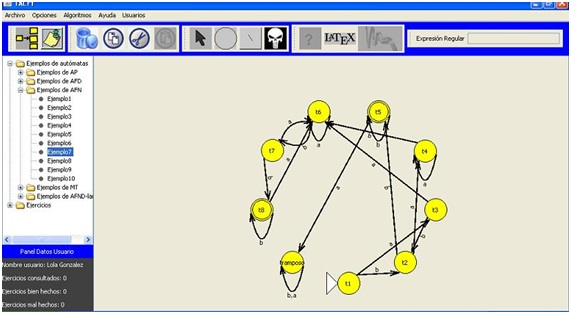
\includegraphics{auto1.jpg}
\end{center}

Y la tabla que obtenemos en el HTML generado cuando queremos ver todos los pasos que hemos seguido en la minimizaci\'on, es la siguiente:

\begin{center}
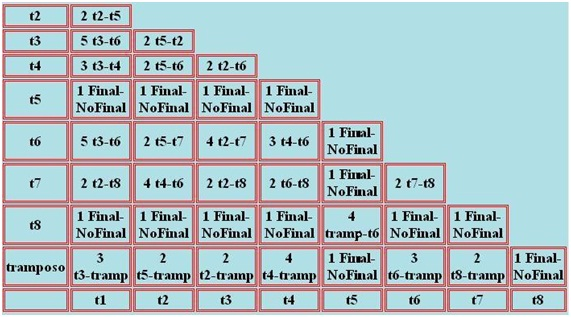
\includegraphics{tabla1.jpg}
\end{center}

En cada celda podemos ver:
\begin{enumerate}
\item Si el estado de la columna es final y el de la fila no final, o viceversa, los dos estados no podr\'an colapsarse, y lo indicamos con Final-No final.

\item A partir de las casillas marcadas con estados que nunca podr\'an colapsarse, procedemos a comprobar que ocurre con el resto de casillas. El n\'umero que aparece nos indica en que ''vuelta'' hemos descubierto que los estados correspondientes a la fila y a la columna no se pueden colapsar. Y para terminar la explicaci\'on de por qu\'e se marca esa casilla, debajo o al lado indicamos que par de estados son los causantes.
\end{enumerate}
Si los estados pudieran colapsarse, la casilla no tendr\'a nada escrito dentro de ella, como ocurre en el ejemplo 10 de aut\'omatas finitos deterministas:

\begin{center}
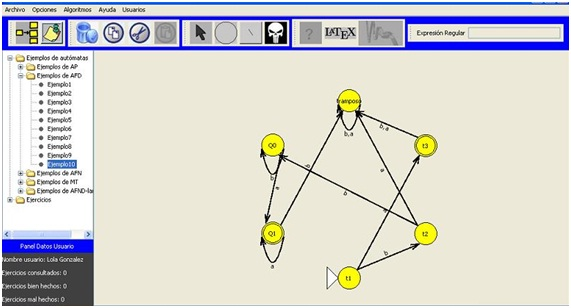
\includegraphics{auto2.jpg}
\end{center}

Cuya tabla de equivalencia es:

\begin{center}
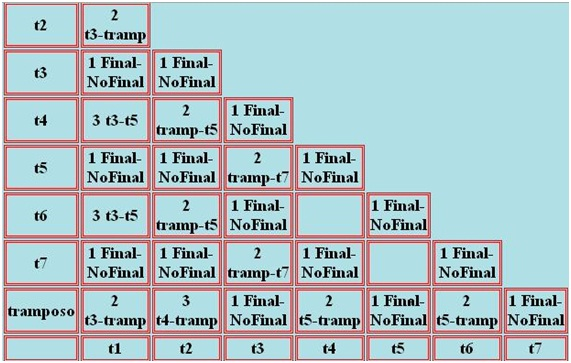
\includegraphics{tabla2.jpg}
\end{center}

Y por \'ultimo, en el HTML dibujamos el aut\'omata resultado de la minimizaci\'on, que ser\'a el mismo que se visualice en la aplicaci\'on.

\begin{center}
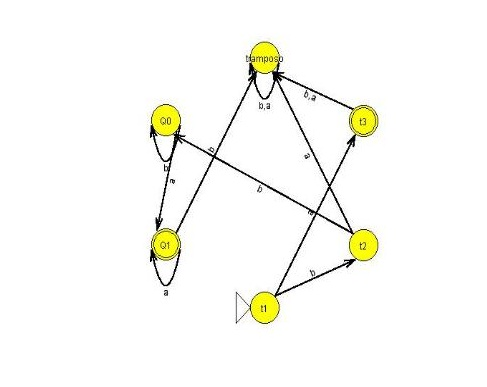
\includegraphics{auto3.jpg}
\end{center}

\newpage
\subsection{Palabras reconocidas por un aut\'omata de pila}
Al tener la aplicaci\'on un enfoque did\'actico, la primera idea que nos vino a la cabeza para saber si una palabra es reconocida por un aut\'omata de pila, fue seguir la misma metodolog\'ia que vimos en clase de TALF. No traduc\'iamos el aut\'omata de pila en una gram\'atica, sino que \'ibamos simulando el comportamiento que ten\'ia el aut\'omata seg\'un iba leyendo los s\'imbolos de la cadena. Conseguimos que este algoritmo funcionase correctamente, siempre que se cumpliera una condici\'on: que el aut\'omata no tuviera ciclos donde solo se lea la cadena vac\'ia sin modificar la pila o a\~nadiendo m\'as s\'imbolos a la misma.

B\'asicamente la idea de funcionamiento de este algoritmo es muy sencilla: Es un algoritmo recursivo, que posee backtracking, pues en muchos casos tenemos m\'as de un camino posible a seguir al procesar una cadena. Si en alg\'un momento, al terminar de consumir los s\'imbolos de la cadena, llegaba a un estado de aceptaci\'on, o se vaciaba la pila, se devolv\'ia un booleano que indicaba que la palabra era aceptada y la se terminaba la ejecuci\'on del algoritmo. En caso contrario, la palabra no se aceptaba y se devolv\'ia falso.
El procedimiento que conten\'ia este algoritmo recibe como par\'ametros:
\begin{enumerate}
\item Lista de estados posibles a los que podemos ir. Tiene prioridad si existe una transici\'on que no consume s\'imbolos. La idea es la siguiente: cuando vamos a procesar el primer s\'imbolo de la cadena, con transiciones vac\'ias es trivial, porque no hemos consumido a\'un ning\'un s\'imbolo, pero si no las hubiera, recopilar\'iamos todos los posibles estados destino, y asumir\'iamos que ya hemos consumido un s\'imbolo de la cadena a reconocer.
\item Pila actual: El estado de la pila hasta el momento. En cada estado al que nos movemos va cambiando, as\'i que solo la modificamos si volvemos a llamar al procedimiento. Si en alg\'un momento se vac\'ia, y si estamos comprobando si la palabra es reconocida por estado, abortamos el procesamiento.
\item N\'umero de elementos que tiene la pila: Inclu\'ido por si en alg\'un momento sirve para detectar los ciclos de los que hemos hablado anteriormente.
\item Cima de la pila en el momento actual: Por comodidad, y por si se quiere comprobar el caso extremo de que si se ha desapilado el s\'imbolo de fondo de pila, y solo queda un s\'imbolo en la pila, pero no coinciden, se pare la simulaci\'on por no poder averiguar, si se ha terminado de vaciar la pila o no. Aqu\'i ser\'ia f\'acil averiguarlo, pero en la teor\'ia de aut\'omatas se restringe de esta manera.
\item Palabra a procesar: Se podr\'ia haber pasado s\'olo como par\'ametro el s\'imbolo actual que se procesa, pero para posibles explicaciones se incluy\'o la palabra completa.
\item \'Indice del s\'imbolo procesado: Se incluye para poder ubicar por cu\'al s\'imbolo de la cadena va la ejecuci\'on.
\item Estado: Estado actual en el que estamos, que nos sirve para poder calcular los posibles movimientos que podemos hacer.
\end{enumerate}


Este procedimiento se apoya en otros dos, que se intuyen seg\'un se ha explicado c\'omo funciona: el primero, que calcula como quedar\'a la pila para la siguiente llamada al procedimiento, y el segundo, que devuelve la lista de posibles estados a los que podemos seguir procesando con un s\'imbolo o no, si es que la transici\'on es vac\'ia, el estado actual, y la cima de pila actual.\\

Quiz\'a en un futuro sean pautas que alguien pueda seguir para explicar el funcionamiento de los aut\'omatas de pila. Nosotros \'ibamos a utilizarlo para probar que una palabra pertenec\'ia al lenguaje de un aut\'omata de pila, pero el coste se disparaba si lo comparamos con el algoritmo llamado CYK, cuyo coste es c\'ubico sobre la longitud de la cadena.

\newpage
\section{Introducci\'on a la ampliaci\'on de la aplicaci\'on}
Repaso a la funcionalidad de TALFi 1.0: \\

TALFi 1.0 es capaz de crear aut\'omatas finitos(deterministas, no deterministas y con transiciones vac\'ias)y expresiones regulares.
Como algoritmos importantes cuenta con la transformaci\'on de un aut\'omata con transiciones vac\'ias a uno no determinista, la transformaci\'on de un aut\'omata no determinista a uno determinista, la transformaci\'on de aut\'omata finito determinista a expresi\'on regular y la minimizaci\'on de aut\'omatas finitos no deterministas.
La interfaz de usuario de TALFi 1.0 cuenta con un \'arbol desplegable donde podemos encontrar ejemplos y ejercicios que la primera versi\'on de TALFi es capaz de llevar a cabo. Tambi\'en dispone de los usuales controles para modificar, copiar, pegar, borrar cualquier aspecto de la figura que creemos en la zona central de la interfaz.

\newpage
\section{Conceptos te\'oricos de la ampliaci\'on}
\subsection{Lenguaje Independiente de Contexto}
Un lenguaje independiente de contexto es aquel generado por una gram\'atica \htmladdnormallink{independiente de contexto.}{http://es.wikipedia.org/wiki/Gramatica_independiente_de_contexto} Estos conceptos pertenecen a un \'area de la Ciencia de la
Computaci\'on llamada Computaci\'on Te\'orica. No hay algoritmo que nos diga el lenguaje
de la gram\'atica, por eso tenemos que ir viendo los s\'imbolos y cadenas que produce.

\subsection{Aut\'omata de Pila}
Un aut\'omata con pila o aut\'omata de pila o aut\'omata a pila o aut\'mata apilador es un
modelo matem\'atico de un sistema que recibe una cadena constituida por s\'imbolos de un
alfabeto y determina si esa \htmladdnormallink{cadena}{http://es.wikipedia.org/wiki/Cadena_de_caracteres} pertenece al \htmladdnormallink{lenguaje}{http://es.wikipedia.org/wiki/Lenguaje_formal} que el aut\'omata reconoce. El
lenguaje que reconoce un \htmladdnormallink{aut\'omata}{http://es.wikipedia.org/wiki/Automata} a pila pertenece al grupo de los \htmladdnormallink{lenguajes de
contexto libre}{http://es.wikipedia.org/wiki/Lenguaje_libre_de_contexto} en la clasificaci\'on de la \htmladdnormallink{Jerarqu\'ia de Chomsky.}{http://es.wikipedia.org/wiki/Jerarquia_de_Chomsky}
\begin{itemize}
\item Definici\'on formal:\\
\newline
Formalmente, un aut\'omata con pila puede ser descrito como una s\'eptupla \\
M = (S,$\Sigma$ ,$\Gamma$ ,$\delta$ ,s,Z,F)
\begin{itemize}
\item $\Sigma$  y $\Gamma$ son alfabetos de entrada, de la cadena y de la pila respectivamente;\\
\item S un conjunto de estados;\\
\item $\delta$: S $\times$ ($\Sigma$ $\cup$ \{$\epsilon$\}) $\times$ $\Gamma$ $\rightarrow$ $\rho$(S $\times$ $\Gamma$*)\\
\item s $\in$ S es el estado inicial;\\
\item Z $\in$ $\Gamma$ es el s\'imbolo inicial de la pila;\\
\item F $\subseteq$ S es un conjunto de estados de aceptaci\'on o finales.\\
\end{itemize}
\newpage
La interpretaci\'on de $\delta$(s,a,Z) = \{($s_{1}$,$\gamma_{1}$),($s_{2}$,$\gamma_{2}$), \ldots ,($s_{n}$,$\gamma_{n}$)\}, con s, $p_{i}$ $\in$ Q, a $\in$ ($\Sigma$ $\cup$ \{$\epsilon$\}), $\gamma_{i}$ $\in$ $\Gamma$ es la siguiente:\\

Cuando el estado del aut\'omata es s, el s\'imbolo que la cabeza lectora est\'a inspeccionando en ese momento es a, y en la cima de la pila nos encontramos el s\'imbolo Z, se realizan las siguientes acciones:\\
\begin{itemize}
\item Si a $\in$ $\Sigma$, es decir no es la palabra vac\'ia, se avanza una posici\'on la cabeza lectora para inspeccionar el siguiente s\'imbolo.
\item Se elimina el s\'imbolo Z de la pila del aut\'omata.
\item Se selecciona un par ($p_{i}$,$\gamma_{i}$)  de entre los existentes en la definici\'on de $\delta$(s,A,Z), la funci\'on de transici\'on del aut\'omata.
\item Se apila la cadena $\gamma_{i}$ = $A_{1}$$A_{2}$\ldots$A_{k}$  en la pila del aut\'omata, quedando el s\'imbolo $A_{1}$  en la cima de la pila.
\item Se cambia el control del aut\'omata al estado $p_{i}$.
\end{itemize}

\item Ejemplo
Sea el siguiente lenguaje libre del contexto L = \{$a^{k}$$b^{k}$ $\mid$ k $\geq$ 0 \}; formado por las cadenas L = \{ $\epsilon$ , ab, aabb, aaabbb, aaaabbbb, \ldots \}\\
\newline
Dicho lenguaje puede ser reconocido por el siguiente aut\'omata con pila:\\
\newline
M = (\{$q_{0}$, $q_{1}$, $q_{2}$, $q_{3}$\}, \{a,b\}, \{A,$\underline{A}$\}, $\delta$, $q_{0}$, \{$q_{0}$, $q_{3}$ \}),
donde las transiciones son:\\
\newline
$\delta$($q_{0}$, a, $\epsilon$) = \{($q_{1}$, $\underline{A}$)\}\\
$\delta$($q_{1}$, a, $\epsilon$) = \{($q_{1}$, $\underline{A}$)\}\\
$\delta$($q_{1}$, b, $\underline{A}$) = \{($q_{2}$, $\epsilon$)\}\\
$\delta$($q_{1}$, b, $\underline{A}$) = \{($q_{3}$, $\epsilon$)\}\\
$\delta$($q_{2}$, b, $\underline{A}$) = \{($q_{2}$, $\epsilon$)\}\\
$\delta$($q_{2}$, b, $\underline{A}$) = \{($q_{3}$, $\epsilon$)\}\\
$\delta$(q, $\theta$, $\rho$) = $\empty$ para cualquier (q,$\theta$,$\rho$)\\

El significado de las transiciones puede ser explicado analizando la primera transici\'on:

$\delta$($q_{0}$, a, $\epsilon$) = \{($q_{1}$, $\underline{A}$)\}

donde q0 es el estado actual, a es el s\'imbolo en la entrada y $\epsilon$ se extrae de la cima de la pila. Entonces, el estado del aut\'omata cambia a q1 y el s\'imbolo $\underline{A}$ se coloca en la cima de la pila.

La idea del funcionamiento del aut\'omata es que al ir leyendo los diferentes s\'imbolos a, estos pasan a la pila en forma de s\'imbolos A. Al aparecer el primer s\'imbolo b en la entrada, se comienza el proceso de desapilado, de forma que coincida el n\'umero de s\'imbolos b le\'idos con el n\'umero de s\'imbolos A que aparecen en la pila.\\
\item Aut\'omata de Pila Determinista:\\
\newline
N\'otese que, a diferencia de un \htmladdnormallink{aut\'omata finito}{http://es.wikipedia.org/wiki/Automata_finito} o una \htmladdnormallink{m\'aquina de Turing}{http://es.wikipedia.org/wiki/Maquina_de_Turing}, la definici\'on b\'asica de un aut\'omata con pila es de naturaleza no determinista, pues la clase de los aut\'omatas con pila deterministas, a diferencia de lo que ocurr\'ia con aquellos modelos, tiene una potencia descriptiva estrictamente menor. Para calificar a un aut\'omata con pila como determinista deben darse dos circunstancias; en primer lugar, por supuesto, que en la definici\'on de cada componente de la funci\'on de transici\'on existan un \'unico elemento lo que da la naturaleza determinista. Pero eso no es suficiente, pues adem\'as puede darse la circunstancia de que el aut\'omata est\'e en el estado s y en la pila aparezca el s\'imbolo sZ, entonces, si existe una definici\'on de transici\'on posible para alg\'un s\'imbolo cualquiera a del alfabeto de entrada, pero, adem\'as existe otra alternativa para la palabra vac\'ia $\epsilon$, tambi\'en esto es una forma de no determinismo, pues podemos optar entre leer un s\'imbolo o no hacerlo. Por eso, en aut\'omata determinista no debe existir transici\'on posible con lectura de s\'imbolo si puede hacerse sin ella, ni al contrario.

Para cada q $\in$ Q, Z $\in$ $\Gamma$, se d\'e que: $\mid$ $\delta$(q,$\epsilon$,Z)$\mid$ + $\mid$ $\delta$(q,a,Z)$\mid$ $\le$ 1 , para cada a $\in$ $\Sigma$.
\end{itemize}

\subsection{Gram\'atica Libre de Contexto}
En ling\"{u}\'istica e inform\'atica, una gram\'atica libre de contexto (o de contexto libre) es una \htmladdnormallink{gram\'atica formal}{http://es.wikipedia.org/wiki/Gramatica_formal} en la que cada regla de producci\'on es de la forma:\\
\newline
    V $\rightarrow$ w\\
\newline
Donde V es un s\'imbolo no terminal y w es una cadena de terminales y/o no terminales. El t\'ermino libre de contexto se refiere al hecho de que el no terminal V puede siempre ser sustituido por w sin tener en cuenta el contexto en el que ocurra. Un \htmladdnormallink{lenguaje formal}{http://es.wikipedia.org/wiki/Lenguaje_formal} es libre de contexto si hay una gram\'atica libre de contexto que lo genera.

Las gram\'aticas libres de contexto permiten describir la mayor\'ia de los lenguajes de programaci\'on, de hecho, la sintaxis de la mayor\'ia de lenguajes de programaci\'on est\'a definida mediante gram\'aticas libres de contexto. Por otro lado, estas gram\'aticas son suficientemente simples como para permitir el dise\~no de eficientes algoritmos de an\'alisis sint\'actico que, para una cadena de caracteres dada determinen como puede ser generada desde la gram\'atica. Los \htmladdnormallink{analizadores LL}{http://es.wikipedia.org/wiki/Analizador_sintactico_LL} y \htmladdnormallink{LR}{http://es.wikipedia.org/wiki/Analizador_sintactico_LR} tratan restringidos subconjuntos de gram\'aticas libres de contexto.

La notaci\'on m\'as frecuentemente utilizada para expresar gram\'aticas libres de contexto es la forma \htmladdnormallink{Backus-Naur.}{http://es.wikipedia.org/wiki/Backus-Naur_form}
\begin{itemize}
\item Defini\'on Formal:\\
As\'i como cualquier gram\'atica formal, una gram\'atica libre de contexto puede ser definida mediante la 4-tupla:\\

G = ($V_{t}$,$V_{n}$,P,S) donde
\begin{itemize}
\item $V_{t}$ es un conjunto finito de terminales
\item $V_{n}$ es un conjunto finito de no terminales
\item P es un conjunto finito de producciones
\item S $\in$ $V_{n}$ el denominado S\'imbolo Inicial
\item los elementos de P son de la forma:\\
        $V_{n}$ $\rightarrow$ ($V_{t}$ $\cup$ $V_{n}$$)^{*}$\\
\end{itemize}

\item Ejemplos:
\begin{enumerate}
\item Una simple gram\'atica libre de contexto es
\begin{center}
    S $\rightarrow$ aSb $\mid$ $\epsilon$\\
\end{center}
donde $\mid$ es un o l\'ogico y es usado para separar m\'ultiples opciones para el mismo no terminal, $\epsilon$ indica una cadena vac\'ia. Esta gram\'atica genera el lenguaje no regular \{$a^{n} b^{n}$: n $\ge$ 0 \} .\\
\item Aqu\'i hay una gram\'atica libre de contexto para expresiones enteras algebraicas sint\'acticamente correctas sobre las variables x, y  y z:
\begin{center}
    S $\rightarrow$ x $\mid$ y $\mid$ z $\mid$ S + S $\mid$ S - S $\mid$ S *S $\mid$ S/S $\mid$ (S)
\end{center}
Generar\'ia, por ejemplo, la cadena (x + y) *x - z *y / (x + x)\\
\item Una gram\'atica libre de contexto para un lenguaje consistente en todas las cadenas que se pueden formar con las letras a y b, habiendo un n\'umero diferente de una que de otra, ser\'ia:\\

    S $\rightarrow$ U $\mid$ V\\
    U $\rightarrow$ TaU $\mid$ TaT\\
    V $\rightarrow$ TbV $\mid$ TbT\\
    T $\rightarrow$ aTbT $\mid$ bTaT $\mid$ $\epsilon$\\

T genera todas las cadenas con la misma cantidad de letras a que b, U genera todas las cadenas con m\'as letras a, y V todas las cadenas con m\'as letras b.\\
\item Otro ejemplo para un lenguaje es \{$a^{n} b^{m} c^{m+n}$: n $\ge$ 0, m $\ge$ 0 \} . No es un lenguaje regular, pero puede ser generado por la siguiente gram\'atica libre de contexto.\\

    S  $\rightarrow$ aSc $\mid$ B
    B $\rightarrow$ bBc $\mid$ E\\
\end{enumerate}
\item Formas normales:
\begin{itemize}
\item Forma Normal de Greibach:\\
\newline
Una gram\'atica independiente del contexto (GIC) est\'a en Forma normal de Greibach (FNG) si todas y cada una de sus reglas de producci\'on tienen un consecuente que empieza por un car\'acter del alfabeto, tambi\'en llamado s\'imbolo terminal. Formalmente, cualquiera de las reglas tendr\'a la estructura:\\
\begin{center}
A $\rightarrow$ aw
\end{center}
Donde ``A'' es el antecedente de la regla, que en el caso de las GIC debe ser necesariamente un solo s\'imbolo auxiliar. Por su parte, ``a'' es el mencionado comienzo del consecuente y, por tanto, un s\'imbolo terminal. Finalmente, ``w'' representa una concatenaci\'on gen\'erica de elementos gramaticales, esto es, una sucesi\'on exclusivamente de auxiliares, inclusive, pudiera ser la palabra vac\'ia; en este caso particular, se tendr\'ia una regla llamada "terminal":\\
\begin{center}
A $\rightarrow$ a
\end{center}
Existe un teorema que prueba que cualquier GIC, cuyo lenguaje no contiene a la palabra vac\'ia, si no lo est\'a ya, se puede transformar en otra equivalente que s\'i est\'e en FNG. Para su demostraci\'on, normalmente, se procede por construcci\'on, es decir, se plantea directamente un algoritmo capaz de obtener la FNG a partir de una GIC dada.\\
\item Forma Normal de Chomsky:\\
\newline
Una gram\'atica formal est\'a en Forma normal de Chomsky si todas sus reglas de producci\'on son de alguna de las siguientes formas:
\begin{center}
A $\rightarrow$ BC \'o\\
A $\rightarrow$ a\\
\end{center}
donde A, B y C son s\'imbolos no terminales (o variables) y a es un s\'imbolo terminal.
Todo lenguaje independiente del contexto que no posee a la cadena vac\'ia, es expresable por medio de una gram\'atica en forma normal de Chomsky (GFNCH) y rec\'iprocamente. Adem\'as, dada una gram\'atica independiente del contexto, es posible algor\'itmicamente producir una GFNCH equivalente, es decir, que genera el mismo lenguaje.
\end{itemize}
\end{itemize}

\subsection{M\'aquina de Turing}
\begin{itemize}
\item Descripci\'on:\\
\newline
La m\'aquina de Turing es un modelo computacional introducido por Alan Turing en el trabajo ``On computable numbers, with an application to the Entscheidungsproblem'', publicado por la Sociedad Matem\'atica de Londres en 1936, en el cual se estudiaba la cuesti\'on planteada por David Hilbert sobre si las matem\'aticas son decidibles, es decir, si hay un m\'etodo definido que pueda aplicarse a cualquier sentencia matem\'atica y que nos diga si esa sentencia es cierta o no. Turing ide\'o un modelo formal de computador, la m\'aquina de Turing, y demostr\'o que exist\'ian problemas que una m\'aquina no pod\'ia resolver. La m\'aquina de Turing es un modelo matem\'atico abstracto que formaliza el concepto de \htmladdnormallink{algoritmo.}{http://es.wikipedia.org/wiki/Algoritmo}\\
\newpage
La m\'aquina de Turing consta de un cabezal lector/escritor y una cinta infinita en la que el cabezal lee el contenido, borra el contenido anterior y escribe un nuevo valor. Las operaciones que se pueden realizar en esta m\'aquina se limitan a:
\begin{center}
\begin{enumerate}
\item avanzar el cabezal lector/escritor hacia la derecha.
\item avanzar el cabezal lector/escritor hacia la izquierda.
\end{enumerate}
\end{center}
El c\'omputo es determinado a partir de una tabla de estados de la forma:
\begin{center}
(estado, valor) $\rightarrow$ (nuevo estado, nuevo valor, direcci\'on)\\
\end{center}
Esta tabla toma como par\'ametros el estado actual de la m\'aquina y el car\'acter le\'ido de la cinta, dando la direcci\'on para mover el cabezal, el nuevo estado de la m\'aquina y el valor a ser escrito en la cinta.

Con este aparato extremadamente sencillo es posible realizar cualquier c\'omputo que un computador digital sea capaz de realizar.

Mediante este modelo te\'orico y el an\'alisis de \htmladdnormallink{complejidad}{http://es.wikipedia.org/wiki/Complejidad_computacional} de algoritmos, fue posible la categorizaci\'on de problemas computacionales de acuerdo a su comportamiento, apareciendo as\'i, el conjunto de problemas denominados \htmladdnormallink{P}{http://es.wikipedia.org/wiki/Tiempo_polinomico} y \htmladdnormallink{NP}{http://es.wikipedia.org/wiki/NP_(Complejidad_computacional)}, cuyas soluciones en tiempo polin\'omico son encontradas seg\'un el determinismo y no determinismo respectivamente de la m\'aquina de Turing.

De hecho, se puede probar matem\'aticamente que para cualquier programa de computadora es posible crear una m\'aquina de Turing equivalente. Esta prueba resulta de la Tesis de Church-Turing, formulada por Alan Turing y Alonzo Church, de forma independiente a mediados del siglo XX.

La idea subyacente es el concepto de que una m\'aquina de Turing es una persona ejecutando un procedimiento efectivo definido formalmente, donde el espacio de memoria de trabajo es ilimitado, pero en un momento determinado s\'olo una parte finita es accesible. La memoria se divide en espacios de trabajo denominados celdas, donde se pueden escribir y leer s\'imbolos. Inicialmente todas las celdas contienen un s\'imbolo especial denominado ``blanco''. Las instrucciones que determinan el funcionamiento de la m\'aquina tienen la forma, ``si estamos en el estado x leyendo la posici\'on y, donde hay escrito el s\'imbolo z, entonces este s\'imbolo debe ser reemplazado por este otro s\'imbolo, y pasar a leer la celda siguiente, bien a la izquierda o bien a la derecha''. La m\'aquina de Turing puede considerarse como un aut\'omata capaz de reconocer lenguajes formales. En ese sentido es capaz de reconocer los lenguajes recursivamente enumerables, de acuerdo a la jerarqu\'ia de Chomsky. Su potencia es, por tanto, superior a otros tipos de aut\'omatas, como el aut\'omata finito, o el aut\'omata con pila, o igual a otros modelos con la misma potencia computacional.\\
\item Definici\'on Formal:\\
\newline
Una m\'aquina de Turing con una sola cinta puede ser definida como una 7-tupla\\
\begin{center}
M=(Q, $\Sigma$, $\Gamma$, s, b, F, $\delta$), donde
\end{center}
\begin{itemize}
\item Q , es un conjunto finito de estados.
\item $\Sigma$, es un conjunto finito de s\'imbolos distinto del espacio en blanco, denominado alfabeto de m\'aquina.
\item $\Gamma$, es un conjunto finito de s\'imbolos de cinta, denominado alfabeto de cinta.
\item $\in$ Q es el estado inicial.
\item $\in$ $\Gamma$ es un s\'imbolo denominado blanco, y es el \'unico s\'imbolo que se puede repetir un n\'umero infinito de veces.
\item F $\subseteq$ Q es el conjunto de estados finales de aceptaci\'on.
\item $\delta$: Q $\times$ $\Gamma$ $\rightarrow$ Q $\times$ $\Gamma$ $\times$ \{I,D,N\}\, es una funci\'on parcial denominada funci\'on de transici\'on, donde I es un movimiento a la izquierda, D es el movimiento a la derecha y N no realiza movimiento alguno.
\end{itemize}
Existen en la literatura un abundante n\'umero de definiciones alternativas, pero todas ellas tienen el mismo poder computacional, por ejemplo se puede a\~nadir el s\'imbolo S como s\'imbolo de ``no movimiento'' en un paso de c\'omputo o el s\'imbolo $\Sigma$ para indicar el alfabeto de entrada.
\newpage
\item Ejemplo:\\
\newline
Definimos una m\'aquina de Turing sobre el alfabeto \{0,1\}, donde 0 representa el s\'imbolo blanco. La m\'aquina comenzar\'a su proceso situada sobre un s\'imbolo ``1'' de una serie. La m\'aquina de Turing copiar\'a el n\'umero de s\'imbolos ``1'' que encuentre hasta el primer blanco detr\'as de dicho s\'imbolo blanco. Es decir, situada sobre el 1 situado en el extremo izquierdo, doblar\'a el n\'umero de s\'imbolos 1, con un 0 en medio. As\'i, si tenemos la entrada ``111'' devolver\'a ``1110111'', con ``1111'' devolver\'a ``111101111'', y sucesivamente.\\
El conjunto de estados es \{$s_1$, $s_2$, $s_3$, $s_4$, $s_5$\} y el estado inicial es $s_1$.\\
\newline
La tabla que describe la funci\'on de transici\'on es la siguiente:\\
\begin{center}
\begin{tabular}{||c|c|c|c|c||}
\hline
Estado & S\'imbolo le\'ido & S\'imbolo escrito & Mov. & Estado sig. \\
\hline
$s_{1}$ & 1 & 0 & D & $s_{2}$ \\
\hline
$s_{1}$ & 1 & 0 & D & $s_{2}$ \\
\hline
$s_{2}$ & 1 & 1 & D & $s_{2}$ \\
\hline
$s_{2}$ & 0 & 0 & D & $s_{3}$ \\
\hline
$s_{3}$ & 0 & 1 & I & $s_{4}$ \\
\hline
$s_{3}$ & 1 & 1 & D & $s_{3}$ \\
\hline
$s_{4}$ & 1 & 1 & I & $s_{4}$ \\
\hline
$s_{4}$ & 0 & 0 & I & $s_{5}$ \\
\hline
$s_{5}$ & 1 & 1 & I & $s_{5}$ \\
\hline
$s_{5}$ & 0 & 1 & D & $s_{1}$ \\
\hline
\end{tabular}
\end{center}
\newpage
El funcionamiento de una computaci\'on de esta m\'aquina se puede mostrar con el siguiente ejemplo (en negrita se resalta la posici\'on de la cabeza lectora/escritora):\\
\begin{center}
\begin{tabular}{||c|c|c||}
\hline
Paso & Estado & Cinta\\
\hline
1 & $s_{1}$ & $\bf{1}$1\\
\hline
2 & $s_{2}$ & 0$\bf{1}$\\
\hline
3 & $s_{2}$ & 01$\bf{0}$\\
\hline
4 & $s_{3}$ & 010$\bf{0}$\\
\hline
5 & $s_{4}$ & 01$\bf{0}$1\\
\hline
6 & $s_{5}$ & 0$\bf{1}$01\\
\hline
7 & $s_{5}$ & $\bf{0}$101\\
\hline
8 & $s_{1}$ & 1$\bf{1}$01\\
\hline
9 & $s_{2}$ & 10$\bf{0}$1\\
\hline
10 & $s_{3}$ & 100$\bf{1}$\\
\hline
11 & $s_{3}$ & 1001$\bf{0}$\\
\hline
12 & $s_{4}$ & 100$\bf{1}$1\\
\hline
13 & $s_{4}$ & 10$\bf{0}$11\\
\hline
14 & $s_{5}$ & 1$\bf{0}$011\\
\hline
15 & $s_{1}$ & 11$\bf{0}$11\\
\hline
Parada & &\\
\hline
\end{tabular}
\end{center}
\newpage
La m\'aquina realiza su proceso por medio de un bucle, en el estado inicial s1, reemplaza el primer 1 con un 0, y pasa al estado s2, con el que avanza hacia la derecha, saltando los s\'imbolos 1 hasta un 0 (que debe existir), cuando lo encuentra pasa al estado s3, con este estado avanza saltando los 1 hasta encontrar otro 0 (la primera vez no habr\'ia ning\'un 1). Una vez en el extremo derecho, a\~nade un 1. Despu\'es comienza el proceso de retorno; con s4 vuelve a la izquierda saltando los 1, cuando encuentra un 0 (en el medio de la secuencia), pasa a s5 que contin\'ua a la izquierda saltando los 1 hasta el 0 que se escribi\'o al principio. Se reemplaza de nuevo este 0 por 1, y pasa al s\'imbolo siguiente, si es un 1, se pasa a otra iteraci\'on del bucle, pasando al estado s1 de nuevo. Si es un s\'imbolo 0, ser\'a el s\'imbolo central, con lo que la m\'aquina se detiene al haber finalizado su c\'omputo.
\end{itemize}
\newpage
\section{Lenguaje generado por un AP}
Esta parte fue la que nos llevo m\'as tiempo, pues como hemos explicado antes, seguimos una l\'inea de trabajo que desafortunadamente nos llevo a un callej\'on sin salida. Nos centramos en palabras que pertenec\'ian al lenguaje, punto importante pero no el vital para el que sirven los aut\'omatas: definir un lenguaje.
\subsection{Algoritmo de paso de AP $\rightarrow$ Gram\'atica}
Encontramos muchas dificultades, pues este algoritmo viene detallado muy formalmente y los ejemplos que pudimos encontrar no eran demasiado aclaratorios.
Para realizar esta nueva funci\'on, hemos incluido en el men\'u de algoritmos el bot\'on ``Simplificaci\'on GIC'':\\
\begin{center}
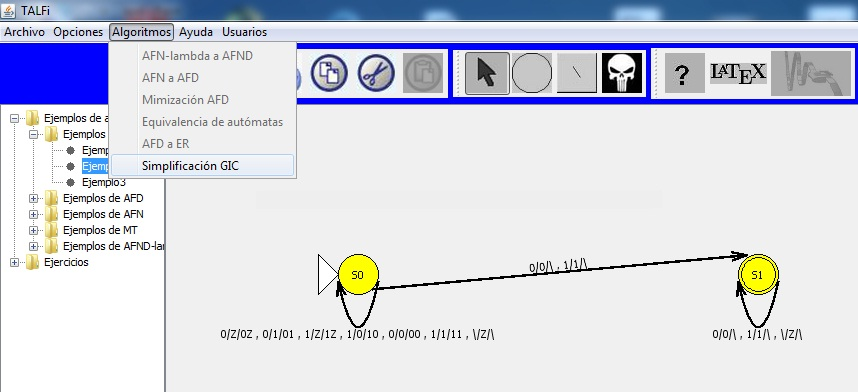
\includegraphics{auto4.jpg}
\end{center}
En primer lugar, tenemos que distinguir si el aut\'omata de pila tiene estados finales o no. Si se da el primer caso, tenemos que convertir el aut\'omata dado en otro equivalente que reconozca el mismo lenguaje por pila vac\'ia que por estado final. Para ello, seguimos el algoritmo que nos dice c\'omo hacerlo:
\begin{itemize}
\item Se debe incluir un nuevo estado inicial y un nuevo fondo de pila. Se a\~nade una transici\'on vac\'ia que vaya al estado inicial antiguo, que apile el antiguo fondo de pila sobre el nuevo.
\newpage
\item Se incluye un nuevo estado, que ser\'a donde se proceda a desapilar todos los s\'imbolos que pudiera haber apilados en el momento de aceptaci\'on de la cadena cuando era aceptada por estado final. Se a\~nade una transici\'on vac\'ia desde cada estado final que desapile para cada s\'imbolo del alfabeto de pila y que vaya al nuevo estado. Por \'ultimo, en este nuevo estado existir\'an aristas con las mismas caracter\'isticas que las anteriores. As\'i, nos aseguramos que, sea posible la transici\'on o no, se desapilar\'ia siempre la pila.\\
\end{itemize}
Podemos verlo m\'as claro en la imagen:\\
\begin{center}
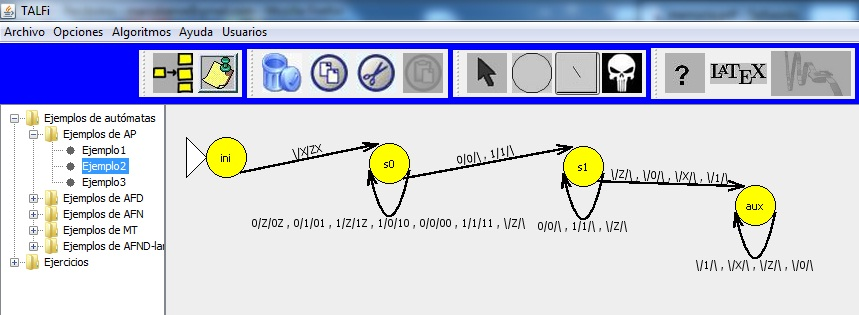
\includegraphics{roci1.jpg}
\end{center}

En ning\'un caso modificamos el aut\'omata que dibuje el usuario, haremos una copia de \'el. Creemos que no es necesario porque es una conversi\'on necesaria para ejecutar el algoritmo, y es bastante intuitivo el cambio, pero si en un futuro se desea se podr\'ia sustituir el original por el nuevo calculado a partir de \'el.\\
\newpage
Una vez que tenemos el aut\'omata libre de estados finales, aplicamos el algoritmo que nos convierte un aut\'omata de pila en una gram\'atica independiente del contexto. Consiste en lo siguiente:
\begin{itemize}
\item El s\'imbolo inicial de la gram\'atica ser\'a S. Para cada estado q del aut\'omata, siendo q0 el estado inicial tendremos la producci\'on\\ S $\rightarrow$ [q0Zq]
\item Si existe una transici\'on tal que desapile la cima de la pila,\\ $\delta$(p,Z,a) = (q, $\epsilon$),
a\~nadimos la producci\'on [pZq] $\rightarrow$ a. Esta a puede ser tambi\'en $\epsilon$.
\item Por \'ultimo, para transiciones $\delta$(p,Z,a) = (q,$A_{1}A_{2}$ \ldots $A_{n}$), debemos construir todas las listas de estados de longitud n, y crear para cada lista la producci\'on:
[pZ$r_{k}$]= a[q$A_{1}r_{1}$][$r_{2}A_{2}r_{3}$] \ldots [$r_{k-1}A_{n}r_{k}$]. Aqu\'i a tambi\'en puede ser $\epsilon$.
\end{itemize}
Una vez que tenemos la gram\'atica, la simplificamos, pues en muchos casos ayuda a reducir los s\'imbolos de variable. Sustituimos todas las variables con producciones unitarias excepto con la variable inicial, y eliminamos las producciones que sean vac\'ias siempre y cuando no aparezcan en S. Para hacer m\'as f\'acil al usuario el entender la gram\'atica, cambiamos los s\'imbolos de producci\'on, que hasta el momento eran del tipo [qZp], por letras may\'usculas del abecedario. Creemos que es bastante grande y que no es probable que ninguna gram\'atica rebase ese n\'umero de variables.
\newpage
\subsection{Algoritmo de simplificaci\'on Gram\'atica tipo 2 a Gram\'atica de Greibach}
Cuando ya tenemos la gram\'atica simplificada podemos dedicarnos a convertirla en una gram\'atica de Greibach. Se caracteriza porque las producciones empiezan por un s\'imbolo terminal, como ya sabemos.\\
Para poder localizar que variables tienen producciones que comiencen por otra variable, construimos una tabla cuyas filas y columnas son las variables de la gram\'atica. Si alguna producci\'on de las variables de las filas comienza con alguna de las variables de las columnas, marcamos la casilla correspondiente.\\
Ve\'amoslo paso por paso, para el ejemplo de la \'ultima imagen:\\

La gram\'atica que nos genera este aut\'omata, es la siguiente:\\
\newline
\begin{center}
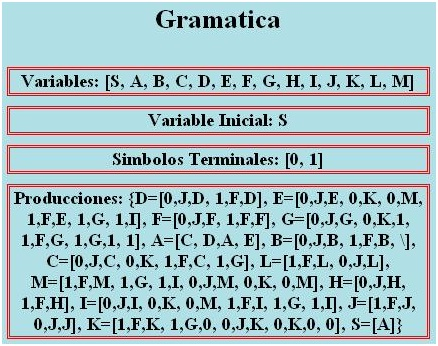
\includegraphics{gram1.jpg}
\end{center}
\newpage
Y la tabla que se genera tal y como hemos dicho antes es la siguiente:\\
\newline
\begin{center}
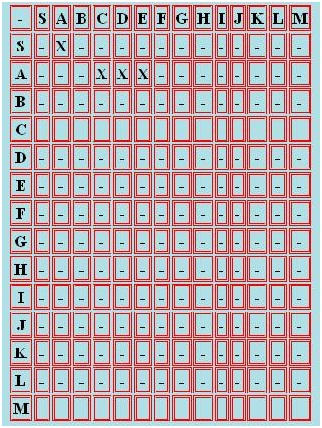
\includegraphics{gram2.jpg}
\end{center}

\newpage
Y mientras que no marquemos una casilla diagonal, es sencillo. Seleccionamos las casillas de la columna m\'as a la izquierda, y sustituimos creando producciones nuevas de la variable marcada en la columna, incluy\'endolas en la variable de la fila. Este proceso es autom\'atico y no se muestra al usuario por pasos, se le vuelve a mostrar la gram\'atica resultante de las sustituciones:\\
\newline
\begin{center}
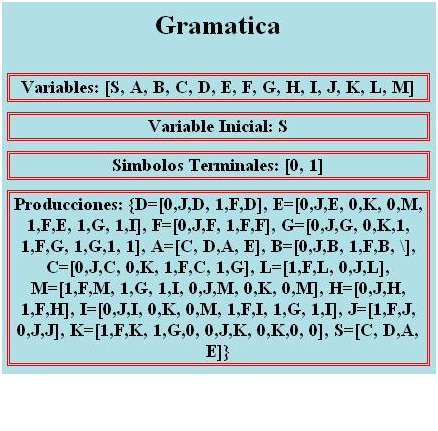
\includegraphics{gram3.jpg}
\end{center}

\newpage
Y volvemos a generar la tabla, hasta que llegamos a un punto que la tabla no est\'a marcada, y eso quiere decir que ya est\'a en forma normal de Greibach.\\
\newline

\begin{center}
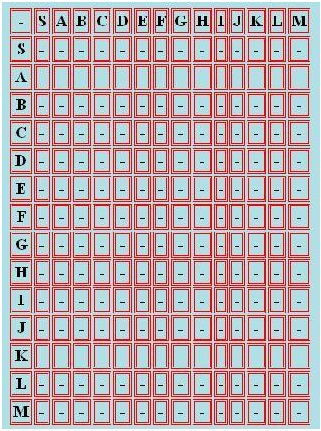
\includegraphics{gram4.jpg}
\end{center}

\newpage
Momento en el que ya hemos terminado y devolvemos la gram\'atica final:\\
\newline
\begin{center}
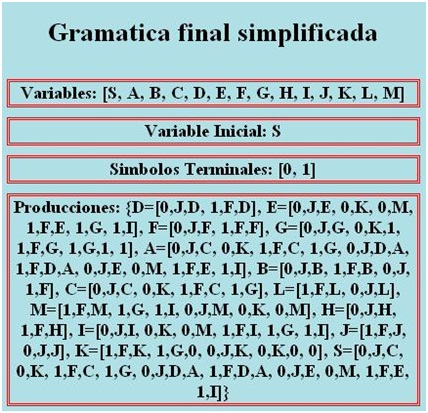
\includegraphics{gram5.jpg}
\end{center}

A esta gram\'atica que devolvemos como final, le aplicamos otro algoritmo de simplificaci\'on, el de eliminar las producciones vac\'ias siempre que no sean producciones de la variable inicial.
Este algoritmo consiste en lo siguiente:
\begin{enumerate}
\item Localizamos que variables, siempre que no sea la inicial, tiene una producci\'on vac\'ia. Eliminamos la producci\'on vac\'ia de sus producciones para cada una de las variables que cumplan esta caracter\'istica.
\item Buscamos en el resto de las producciones de las variables si existe alguna que contenga la variable con la producci\'on vac\'ia. La sustituimos, y la a\~nadimos a la lista de producciones.
\end{enumerate}
Consideramos que cuando la tabla no contiene marcas es el momento ideal de proceder a eliminarlas, porque si lo hacemos antes de que est\'e en Forma Normal de Greibach, no podemos asegurar que entremos en un bucle infinito y no podamos salir de \'el. Por ejemplo:\\
Tenemos dos producciones del tipo:\\
\begin{center}
A $\rightarrow$ \ldots $\mid$ E $\mid$ $\epsilon$ $\mid$ \ldots\\
E $\rightarrow$ \ldots $\mid$ A $\mid$ \ldots\\
\end{center}
Siendo A, E variables de la gram\'atica. Si eliminamos las producciones vac\'ias, ocurrir\'ia lo siguiente:\\
\begin{enumerate}	
\item Sustituimos  las apariciones de A por $\epsilon$. Obtendr\'iamos lo siguiente:\\
\begin{center}
	A $\rightarrow$ \ldots $\mid$ E $\mid$ \ldots\\
	E $\rightarrow$ \ldots $\mid$ $\epsilon$ $\mid$ \ldots\\
\end{center}
\item Volver\'iamos a estar en la misma situaci\'on, pues seguimos teniendo una variable con una producci\'on vac\'ia.
\end{enumerate}
Este problema no lo tenemos si la gram\'atica tiene la Forma Normal de Greibach, pues nos aseguramos que el primer s\'imbolo de la producci\'on es un terminal, y nunca ocurrir\'a el caso anterior.

Por otro lado, puede ocurrir que se marque una casilla que est\'e en la diagonal de la tabla. En ese caso el proceso es algo m\'as delicado, pues hemos de incluir una nueva variable, ya que existe recursividad y por mucho que se sustituya una y otra vez no podr\'iamos eliminarla.
%Pong\'amonos en esta situaci\'on. Tenemos esta gram\'atica:

%(NO ENCUENTRO EJEMPLOS CON DIAGONAL CON AUTOMATAS!!!!!)

%Cuya tabla es esta:

%(NO ENCUENTRO EJEMPLOS CON DIAGONAL CON AUTOMATAS!!!!!)

%Pues, lo que tenemos que hacer ahora es (NO RECUERDO MIRAR MA\~NANA LIBRO AZUL!)
\newpage
\subsection{Algoritmo de simplificaci\'on de gram\'atica de tipo 2 a gram\'atica de Chomsky}
Ya que hemos incluido simplificaciones de gram\'atica, no podemos no incluir otras de las simplificaciones, quiz\'a m\'as importante incluso que la Forma Normal de Greibach: La Forma Normal de Chomsky.\\
\newline
Convertir una gram\'atica en Forma Normal de Chomsky, consiste en dos pasos muy sencillos. En primer lugar, una gram\'atica est\'a en forma normal de Chomsky si las producciones son del tipo:
\begin{center}
A $\rightarrow$ BC 	Siendo A, B, C $\in$ V\\
A $\rightarrow$ a        Siendo a $\in$  T
\end{center}
Y s\'olo se puede incluir la producci\'on S $\rightarrow$ $\epsilon$ si S no aparece en ninguna de las producciones del resto de variables y, por supuesto,  aparece en los casos que \'unicamente $\epsilon$ es reconocida por la gram\'atica.\\
\newline
Con esta idea en la cabeza, es f\'acilmente entendible el algoritmo de transformaci\'on, que consta de dos fases:
\begin{itemize}
\item Fase 1: Para cada s\'imbolo terminal que pertenece a T, creamos producciones del tipo [Ca] $\rightarrow$ a
para todo a $\in$ T.
\begin{itemize}
\item Fase 1.1: Reemplazamos en todas las producciones las apariciones de s\'imbolos terminales  a por sus ``variables terminales'' [Ca] asociados que acabamos de crear.
\end{itemize}
\item Fase 2: Ahora tenemos que conseguir que las producciones est\'en formadas solamente por dos variables. Para ello procedemos de la siguiente manera:
\begin{itemize}
\item Fase 2.2: Recorremos todas las producciones. Si la longitud es mayor o igual a 3, esto es lo que hacemos:\\
Imaginemos que tenemos la siguiente producci\'on: A $\rightarrow$ $A_{1}A_{2}A_{3} \ldots A_{n}$. Creamos una nueva variable, [D0], que contendr\'a la producci\'on $A_{2}A_{3} \ldots A_{n}$, y modificamos la producci\'on que acabamos de encontrar suplant\'andola por A$\rightarrow$ $A_{1}$[D0].
\end{itemize}
	Esta fase 2 se repite hasta que todas las producciones tengan longitud menor que 3, o lo que es lo mismo, que ninguna cumpla la condici\'on para ser modificada.\\
\newline
En teor\'ia habr\'iamos acabado aqu\'i, pero puede ocurrir, que la gram\'atica original, tuviera producciones de s\'olo una variable, y entonces no estar\'ia la forma normal de Chomsky bien construida.\\ Este detalle en el algoritmo no se tiene en cuenta, pero es lo que nos ha ocurrido a lo largo de todo este a\~no trabajando en el proyecto:\\ las diferencias entre las aplicaciones te\'oricas, y lo que en la pr\'actica supone estudiar todos los casos, no \'unicamente el general, y buscar soluciones eficientes para devolver el resultado correcto. As\'i que, informalmente, a\~nadir\'iamos un tercer paso:
\item Fase 3: Si en alg\'un momento encontramos en las producciones alguna que consista en una variable, sustituimos esa variable por todas sus producciones, pues en principio tendr\'an la forma adecuada que requiere la Forma Normal de Chomsky. Y finalmente diremos que la gram\'atica est\'a simplificada en el momento que hayamos revisado todas las producciones y no hayamos hecho ninguna modificaci\'on.
\end{itemize}
A continuaci\'on, vamos a mostrar cu\'al es el resultado de obtener la Forma Normal de Chomsky en un aut\'omata sencillo:\\
\begin{center}
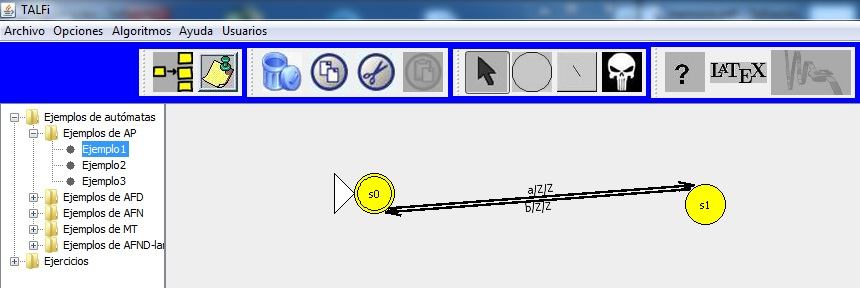
\includegraphics{chom1.jpg}
\end{center}

Y la salida HTML mostrada con su Forma Normal de Chomsky, que tiene un formato id\'entico a la salida de la Forma Normal de Greibach excepto en los pasos que sigue para llegar al resultado final, es la siguiente:\\
\newpage
\begin{enumerate}
\item Lo primero, saber cu\'al es la gram\'atica primigenia:\\
\begin{center}
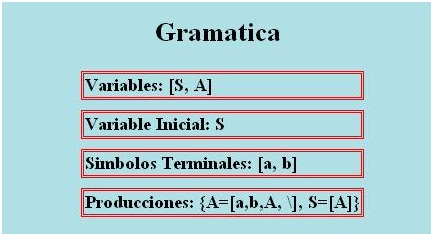
\includegraphics{chom2.jpg}
\end{center}
\item La salida obtenida de aplicar la primera fase, cuyo resultado es claramente intuitivo compar\'andolo con la gram\'atica original:\\
\begin{center}
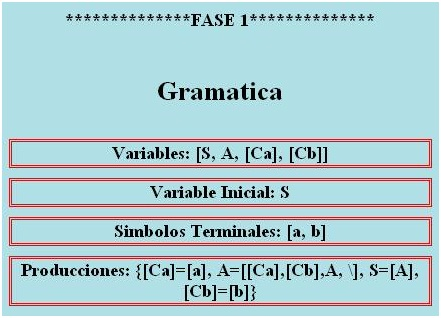
\includegraphics{chom3.jpg}
\end{center}
\newpage
\item La salida obtenida de terminar con la segunda fase:\\
\begin{center}
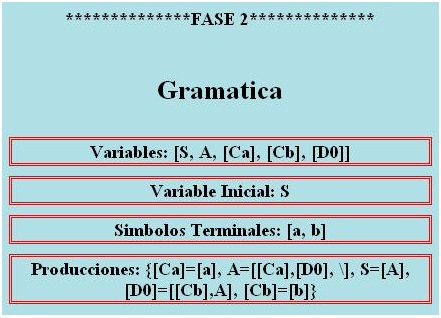
\includegraphics{chom4.jpg}
\end{center}
\item Observemos la producci\'on S $\rightarrow$ A y la producci\'on de [D0] c\'omo cambia al terminar con la simplificaci\'on y conseguir una gram\'atica en Forma Normal de Chomsky:\\
\begin{center}
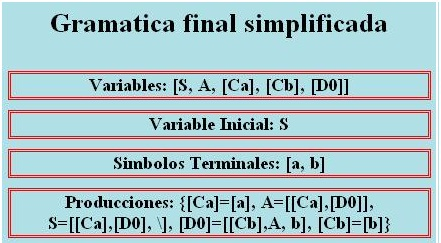
\includegraphics{chom5.jpg}
\end{center}
\end{enumerate}

\newpage
\subsection{Generaci\'on aleatoria de palabras}
Como ya sabemos, los aut\'omatas de pila definen lenguajes. El uso de la pila dificulta en algunos casos saber c\'omo son las cadenas reconocidas, por tanto implementamos una manera de conseguir una lista que mostrase algunas de las palabras reconocidas.
Esta lista contiene como m\'aximo cinco palabras. En un primer momento pensamos en que tuviera diez, pero para gram\'aticas con muchas variables, es muy probable que tengan muchas producciones para cada una de ellas, aumentando considerablemente el coste y el uso de memoria.
Despu\'es de tener esta informaci\'on, cogemos las producciones de la variable inicial, y creamos una lista donde iremos guardando las derivaciones por la izquierda que podr\'iamos construir con la gram\'atica. Y a partir de aqu\'i, el algoritmo consiste en lo siguiente:\\
\newline
Mientras que la lista de palabras construidas no llegue a cinco, haremos lo siguiente:
\begin{itemize}
\item Cogemos la primera derivaci\'on de la producci\'on y la eliminamos de la lista.
\item Si est\'a formada solamente por s\'imbolos terminales, la eliminamos de la lista y la metemos en la lista de palabras reconocidas por el aut\'omata.
\item Si no, buscamos el primer s\'imbolo de variable que aparezca por la izquierda. En caso de que esa variable pertenezca a la lista que calculamos antes de variables con producciones que son un terminal, la sustituimos por todas las producciones que tenga de ese tipo, y se a\~naden las diferentes derivaciones resultantes para cada sustituci\'on.
\end{itemize}
La longitud de la lista es un par\'ametro f\'acilmente modificable para futuras mejoras de la aplicaci\'on, pues est\'a definida como una constante. Consideramos no dejarla a la elecci\'on del usuario, porque la idea de mostrar esta lista es que el usuario tenga una ligera intuici\'on del lenguaje generado por el aut\'omata, animando a que sea \'el mismo el que profundice en las cadenas que pertenecen al lenguaje y tambi\'en en las que no.

\newpage
\section{M\'aquinas de Turing}
\subsection{Nociones preliminares}
El modelo de m\'aquina de Turing es equivalente en cuanto a potencia de c\'omputo a un ordenador.
Las m\'aquinas de Turing han acabado siendo una definici\'on formal aceptada de algoritmo. Lo que no pueda computar ninguna m\'aquina de Turing no es computable.
Por tanto, la potencia de estos aut\'omatas no es superable.\\

\begin{center}
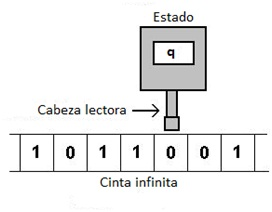
\includegraphics{turi1.jpg}
\end{center}

Alain Turing se plante\'o formalizar el comportamiento humano (como computadora) al usar l\'apiz y papel para resolver un problema mediante un algoritmo.\\
Para ello descompuso todo en procesos muy simples:\\
\begin{itemize}
\item Un n\'umero finito de estados mentales (Q).
\item Papel cuadriculado, cinta potencialmente infinita dividida en celdas.
\item En un mismo paso de c\'omputo podemos:
\begin{enumerate}
\item Cambiar de estado (mental).
\item Alterar el contenido de la casilla de trabajo (borrar o escribir).
\item Concentrarnos en otra casilla (la misma, derecha o izquierda).
\end{enumerate}
\end{itemize}
Con esta definici\'on y sabiendo que un lenguaje es reconocido por una m\'aquina de Turing cuando:
\begin{center}
L(M) = \{x $\in$ $A^{*}$ $\mid$ M acepta  a x\}
\end{center}
Se ha creado un algoritmo para TALFi, el cual, dada una palabra y un aut\'omata que representa a una m\'aquina de Turing, nos dice si dicha palabra es reconocida por la m\'aquina.

Para ello, se coloca la palabra en un archivo de texto (para poder trabajar de la manera m\'as parecida posible a una cinta con celdas infinitas), y se le pasa al algoritmo como argumento para que compruebe la palabra en cuesti\'on.

\subsection{Algoritmo de reconocimiento}
Una vez comprendida la formalizaci\'on de Turing, la hemos usado de una manera muy intuitiva, para comprobar si la palabra que introducimos puede ser reconocida por el lenguaje que denota la m\'aquina de Turing dise\~nada.

Una vez hemos dise\~nado una m\'aquina de Turing en el \'area espec\'ifica para ello en TALFi, disponemos de un bot\'on con el cual abrir el archivo de texto que contiene la palabra a tratar.

\begin{center}
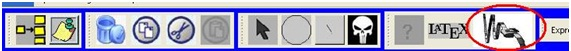
\includegraphics{turi2.jpg}
\end{center}

Una vez pulsado el bot\'on, se abrir\'a el usual di\'alogo de apertura de archivos. Seleccionado el archivo, el algoritmo pasa a realizar los siguientes pasos:
\begin{enumerate}
\item Busca el primer estado para iniciar el procesamiento de la cinta (archivo de texto).
\item Coloca la cabeza lectora al principio de la cinta (primer s\'imbolo que no es un blanco).
\item Analiza que transici\'on entre las existentes en la m\'aquina, contienen el estado inicial y el car\'acter actual de la cabeza lectora.
\item Si existe la transici\'on, actualiza el valor de la celda de la cinta y se desplaza a la celda que indique la propia transici\'on (N =  no se desplaza, I = izquierda, D = derecha. Si no existe, la palabra no ser\'a reconocida, mostrando en el archivo de texto dicha situaci\'on.
\item Vuelve al paso 3 para ver si la nueva transici\'on existe (pero ahora con el estado y el s\'imbolo de cinta actualizados) y en caso afirmativo, tratarla de la misma manera, modificando la cinta.
\item Si al final de todo el c\'omputo, la palabra resulta reconocida, la salida que se ofrecer\'a en la cinta (archivo de texto) de la m\'aquina de Turing (por definici\'on) ser\'a la celda que se encuentra inmediatamente a la derecha de la \'ultima posici\'on de la cinta de entrada que no es un blanco de cinta.
\end{enumerate}

\subsection{Ampliaciones y problemas}
No hemos mencionado en la anterior descripci\'on del algoritmo, el caso en el que una m\'aquina de Turing, no acabe nunca su c\'omputo, es decir, cicle o no sea terminante.
Este problema no es decidible, ni siquiera existe una m\'aquina de Turing para esto.
Por ello recurrimos a una idea que si bien no ser\'a capaz de solucionar todos los casos, si un alto porcentaje de ellos.
Supongamos una m\'aquina de Turing y una palabra x dada, dicha m\'aquina puede:
\begin{itemize}
\item Aceptar a x, si existe una configuraci\'on de parada y aceptadora.
\item Rechazar a x, si existe una configuraci\'on de parada y no aceptadora.
\item Ciclar, si no existe una configuraci\'on de parada.
\end{itemize}
Dado que en un principio este problema no fue contemplado, era necesario a\~nadir alg\'un tipo complemento para que se detectase el caso de ciclo en el c\'omputo de una m\'aquina de Turing. Dicho complemento, es una cota que utilizan varios algoritmos conocidos. Dicha cota est\'a relacionada con la longitud de la cinta y el n\'umero de transiciones de la m\'aquina de Turing  y su tratamiento consiste en consultar el n\'umero de transiciones visitadas hasta el momento y compararlas con dicha cota.

\newpage
\section{Ejercicios}
Ahora tambi\'en es posible crear ejercicios de aut\'omatas de pila y m\'aquinas de Turing. Hemos incluido una peque\~na colecci\'on, pero el administrador puede ampliarla creando sus propios ejercicios y a\~nadi\'endolos a la base de datos de los mismos. A continuaci\'on detallaremos como crearlos, que informaci\'on interna generan, y la forma de corregirlos que hemos implementado.\\
\subsection{Cambios en la interfaz gr\'afica e implementaci\'on interna para ejercicios de Aut\'omatas de Pila y M\'aquinas de Turing}
Hasta el momento, el administrador solamente ten\'ia que escribir el aut\'omata o la expresi\'on regular que fuera soluci\'on, y el enunciado del ejercicio.\\
\newline
Para los nuevos ejercicios necesitamos m\'as informaci\'on para poder asegurar que la soluci\'on que proporcione el usuario es la suministrada por el administrador de la aplicaci\'on. Por este motivo, ahora se pueden suministrar dos listas de palabras, en el caso de aut\'omatas de pila, y una en el caso de Turing.\\
\newline
Se siguen creando de la misma manera que los anteriores ejercicios,\\ seleccion\'andolos de la lista de todos los posibles:\\
\begin{center}
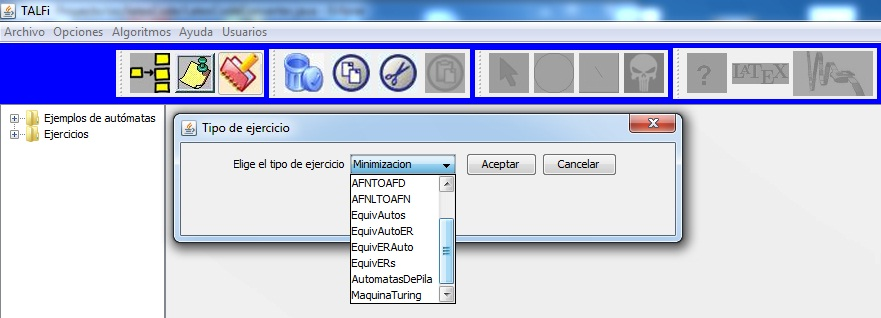
\includegraphics{ejer1.jpg}
\end{center}
\newpage
Una contendr\'a las palabras que han de ser reconocidas o procesadas, y otra que contendr\'a palabras que deben ser rechazadas. Ninguna de las dos tiene l\'imite.  Al aut\'omata que pinte el usuario se le aplicar\'a el algoritmo de CYK en el caso de los aut\'omatas de pila, y si coinciden todos los resultados, se considerar\'a el ejercicio como apto, en otro caso no se dar\'a como v\'alido.\\
\begin{center}
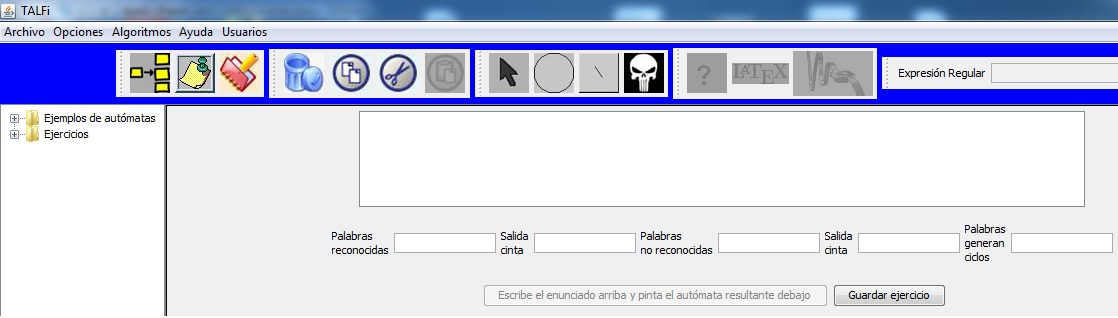
\includegraphics{ejer2.jpg}
\end{center}

En Turing s\'olo consideramos una lista, porque si las cadenas no son aceptadas no podemos asegurar que la m\'aquina pare. Internamente se simular\'a la salida de la cinta cuando la m\'aquina se detenga, y se comparar\'a con la salida de la cinta de la m\'aquina que proporcione el usuario. En caso de que coincidan, ocurre como en el otro tipo de ejemplos, se consideran aptos, y no aptos en otro caso.

\chapter{Anexos}
\section{\LaTeX{}}

La opci\'on de que TALFi imprimiese cualquier aut\'omata que se dibujase en {\LaTeX{}} o mostrase los pasos de una simplificaci\'on de gram\'aticas en dicho formato, no fue uno de los riquisitos de la especificaci\'on en un principio.\\
Pero la opci\'on concedida gracias a una beca del PIE (Programa de Iniciaci\'on a la Empresa), nos dio la oportunidad de a\~nadir esta funcionalidad a la aplicaci\'on y poder trabajar con este formato de texto tan usado entre profesionales.\\
\subsection{Introducc\'on a \LaTeX{}}
\LaTeX{} es un sistema de composici\'on de textos, orientado especialmente a la creaci\'on de libros, documentos cient\'ificos y t\'ecnicos que contengan f\'ormulas matem\'aticas.

\LaTeX{} est\'a formado por un gran conjunto de macros de \TeX{}, escrito por Leslie Lamport en 1984, con la intenci\'on de facilitar el uso del lenguaje de composici\'on tipogr\'afica \TeX{}, creado por Donald Knuth. Es muy utilizado para la composici\'on de art\'iculos acad\'emicos, tesis y libros t\'ecnicos, dado que la calidad tipogr\'afica de los documentos realizados con \LaTeX{} es comparable a la de una editorial cient\'ifica de primera l\'inea.

\LaTeX{} es software libre bajo licencia LPPL.

\newpage
\subsection{Descripci\'on:}
\LaTeX{} es un sistema de composici\'on de textos que est\'a formado mayoritariamente por \'ordenes (macros) construidas a partir de comandos de \TeX{} ---un lenguaje ``de bajo nivel'', en el sentido de que sus acciones \'ultimas son muy elementales--- pero con la ventaja a\~nadida, en palabras de Lamport, de ``poder aumentar las capacidades de \LaTeX{} utilizando comandos propios del \TeX{} descritos en The TeXbook''. Esto es lo que convierte a \LaTeX{} en una herramienta pr\'actica y \'util pues, a su facilidad de uso, se une toda la potencia de \TeX{}. Estas caracter\'isticas hicieron que \LaTeX{} se extendiese r\'apidamente entre un amplio sector cient\'ifico y t\'ecnico, hasta el punto de convertirse en uso obligado en comunicaciones y congresos, y requerido por determinadas revistas a la hora de entregar art\'iculos acad\'emicos.

Su c\'odigo abierto permiti\'o que muchos usuarios realizasen nuevas utilidades que extendiesen sus capacidades con objetivos muy variados, a veces ajenos a la intenci\'on con la que fue creado: aparecieron diferentes dialectos de \LaTeX{} que, a veces, eran incompatibles entre s\'i. Para atajar este problema, en 1989 Lamport y otros desarrolladores iniciaron el llamado ``Proyecto LaTeX3''. En oto\~no de 1993 se anunci\'o una reestandarizaci\'on completa de \LaTeX{}, mediante una nueva versi\'on que inclu\'ia la mayor parte de estas extensiones adicionales (como la opci\'on para escribir transparencias o la simbolog\'ia de la American Mathematical Society) con el objetivo de dar uniformidad al conjunto y evitar la fragmentaci\'on entre versiones incompatibles de \LaTeX{} 2.09. Esta tarea la realizaron Frank Mittlebach, Johannes Braams, Chris Rowley y Sebastian Rahtz junto al propio Leslie Lamport. Hasta alcanzar el objetivo final del ``Proyecto 3'', a las distintas versiones se las viene denominando \LaTeX{}$2_\epsilon$ (o sea, ``versi\'on 2 y un poco m\'as...''). Actualmente cada a\~no se ofrece una nueva versi\'on, aunque las diferencias entre una y otra suelen ser muy peque\~nas y siempre bien documentadas.

Con todo, adem\'as de todas las nuevas extensiones, la caracter\'istica m\'as relevante de este esfuerzo de reestandarizaci\'on fue la arquitectura modular: se estableci\'o un n\'ucleo central (el compilador) que mantiene las funcionalidades de la versi\'on anterior pero permite incrementar su potencia y versatilidad por medio de diferentes paquetes que solo se cargan si son necesarios. De ese modo, \LaTeX{} dispone ahora de innumerables paquetes para todo tipo de objetivos, muchos dentro de la distribuci\'on oficial, y otros realizados por terceros, en algunos casos para usos especializados.

\subsection{Uso}
\LaTeX{} presupone una filosof\'ia de trabajo diferente a la de los procesadores de texto habituales (conocidos como WYSIWYG, es decir, ``lo que ves es lo que obtienes'') y se basa en comandos. Tradicionalmente, este aspecto se ha considerado una desventaja (probablemente la \'unica). Sin embargo, \LaTeX{}, a diferencia de los procesadores de texto de tipo WYSIWYG, permite a quien escribe un documento centrarse exclusivamente en el contenido, sin tener que preocuparse de los detalles del formato. Adem\'as de sus capacidades gr\'aficas para representar ecuaciones, f\'ormulas complicadas, notaci\'on cient\'ifica e incluso musical, permite estructurar f\'acilmente el documento (con cap\'itulos, secciones, notas, bibliograf\'ia, \'indices anal\'iticos, etc.), lo cual brinda comodidad y lo hace \'util para art\'iculos acad\'emicos y libros t\'ecnicos.\\

Con \LaTeX{}, la elaboraci\'on del documento requiere normalmente de dos etapas: en la primera hay que crear mediante cualquier editor de texto llano un fichero fuente que, con las \'ordenes y comandos adecuados, contenga el texto que queramos imprimir. La segunda consiste en procesar este fichero; el procesador de textos interpreta las \'ordenes escritas en \'el y compila el documento, dej\'andolo preparado para que pueda ser enviado a la salida correspondiente, ya sea la pantalla o la impresora. Ahora bien, si se quiere a\~nadir o cambiar algo en el documento, se deber\'a hacer los cambios en el fichero fuente y procesarlo de nuevo. Esta idea, que puede parecer poco pr\'actica a priori, es conocida a los que est\'an familiarizados con el proceso de compilaci\'on que se realiza con los lenguajes de programaci\'on de alto nivel (C, C++, etc.), ya que es completamente an\'alogo.\\

El modo en que \LaTeX{} interpreta la ``forma'' que debe tener el documento es mediante etiquetas. Por ejemplo, ``documentclass\{article\}'' le dice a \LaTeX{} que el documento que va a procesar es un art\'iculo. Puede resultar extra\~no que hoy en d\'ia se siga usando algo que no es WYSIWYG, pero las caracter\'isticas de \LaTeX{} siguen siendo muchas y muy variadas. Tambi\'en hay varias herramientas (aplicaciones) que ayudan a una persona a escribir estos documentos de una manera m\'as visual (LyX, TeXmacs y otros). A estas herramientas se les llama WYSIWYM (``lo que ves es lo que quieres decir'').\\
\newpage
Una de las ventajas de \LaTeX{} es que la salida que ofrece es siempre la misma, con independencia del dispositivo (impresora, pantalla, etc.) o el sistema operativo (MS Windows, MacOS, Unix, GNU/Linux, etc.) y puede ser exportado a partir de una misma fuente a numerosos formatos tales como Postscript, PDF, SGML, HTML, RTF, etc. Existen distribuciones e IDEs de LaTeX para todos los sistemas operativos m\'as extendidos, que incluyen todo lo necesario para trabajar. Hay, por ejemplo, programas para Windows como TeXnicCenter, \htmladdnormallink{MikTeX}{http://miktex.org/} o \htmladdnormallink{WinEdt}{http://www.winedt.com/}, para Linux como Kile, o para MacOS como TeXShop, todos liberados bajo la Licencia GPL. Existe adem\'as un editor multiplataforma (para MacOS, Windows y Unix) llamado Texmaker, que tambi\'en tiene licencia \htmladdnormallink{GPL}{http://es.wikipedia.org/wiki/Licencia_publica_general_de_GNU}.

\subsection{Uso de \LaTeX en la herramienta TALFi}
Aunque \LaTeX es primordialmente un sistema de composici\'on de textos para la creaci\'on de documentos que contengan f\'ormulas matem\'aticas, en TALFi lo usaremos para poder colocar en nuestros textos aut\'omatas o simplificaciones paso a paso de gram\'aticas.

Esto es posible debido a una gran cantidad y diversidad de bibliotecas/paquetes que podemos a\~nadir a nuestro editor de \LaTeX{}.
Gracias a esta amplitud de posibilidades para crear gr\'aficos complejos en \LaTeX{}, el trabajo inicial de poder imprimir los aut\'omatas o las simplificaciones acab\'o dando como resultado 3 posibles representaciones en \LaTeX{}. De esta manera y debido a las diferencias entre las representaciones, el usuario podr\'a elegir entre un dise\~no sobrio y con formas claras, un dise\~no colorido o un dise\~no en forma matricial para poder modificarlo de manera m\'as intuitiva.

Sin embargo para la representaci\'on de los pasos en la simplificaci\'on de gram\'aticas, s\'olo disponemos de un dise\~no, puesto que la representaci\'on se hace mediante tablas y texto plano, siendo innecesaria la inclusi\'on de colores, formas, etc.
\newpage
\subsection{LatexCodeConverter}
Esta clase, es la encargada de traducir cualquier aut\'omata de TALFi en un archivo \TeX{} totalmente listo para ser compilado en cualquier entorno para \LaTeX{}.
\newline
\begin{itemize}
\item Algoritmo conversor:\\
\newline
La implementaci\'on del algoritmo consiste b\'asicamente en traducir los distintos campos de los que consta un aut\'omata en comandos \LaTeX{}:
\begin{enumerate}
\item Para cada estado del aut\'omata se crea un c\'irculo en el que dentro se incluye su etiqueta. Se detectan el estado inicial y los de aceptaci\'on, para los que se usan otra representaci\'on, adem\'as de su c\'irculo.
\item Se toma cada coordenada de cada nodo del aut\'omata TALFi para colocarlo de la misma manera en el archivo que generemos con \LaTeX{}.
\item Generamos las aristas viendo desde que estado parten y a cual se dirigen.
\item Cerramos el archivo.\\
\end{enumerate}
\newpage
\item Representaciones:\\
\begin{enumerate}
\item Mediante biblioteca xy:\\
\newline
Esta es la representaci\'on m\'as fiable y visualmente m\'as clara, puesto que siempre que se pueda dibujar un aut\'omata en TALFi, su representaci\'on en \LaTeX ser\'a pr\'acticamente id\'entica.\\
\begin{center}
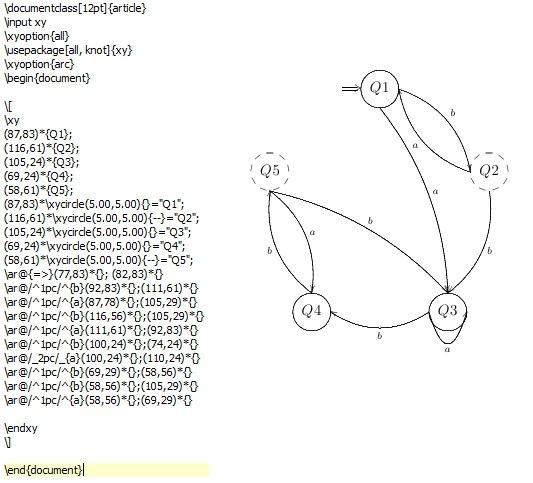
\includegraphics{late1.jpg}
\end{center}

\newpage
\item Mediante biblioteca TikZ:\\
\newline
Esta biblioteca es visualmente muy atractiva, pero tiene el incoveniente de que el modo en el que los estados se colocan en el lienzo, se realiza especificando donde se encuentran cada uno de ellos, en relaci\'on a un estado dado.
Como vemos en el c\'odigo, partimos del estado A ($q_{a}$ en el dibujo), para luego indicar que el estado B se encuentra arriba y a la derecha del estado A. Lo mismo ocurre con el estado C, que se indica que est\'a abajo y a la derecha del estado B,etc.\\
\newline
Aunque visualmente gane muchos enteros este tipo de representaci\'on, debido a que el algoritmo construye el dibujo de manera de autom\'atica, puede llevar a muchos problemas de superposici\'on de estados cuando los aut\'omatas contienen un n\'umero de estados elevado (inlcuso pord\'ia no poder visualizarse).\\
Conllevar\'ia una trabajo dificultoso de grafos para llevar a cabo una representaci\'on de aut\'omatas totalmente libre de errores para esta representaci\'n.
No obstante, si se quieren incluir aut\'omatas en un texto \LaTeX{} de manera manual, este es el mejor m\'etodo posible.\\
\newline
Lo comprobamos en un ejemplo:
\begin{center}
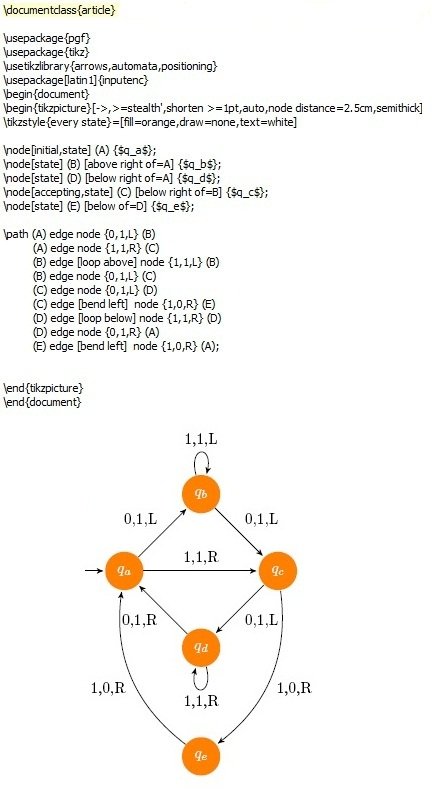
\includegraphics{late2.jpg}
\end{center}


\item Mediante biblioteca Psmatrix:\\
\newline
En esta implementaci\'on, no cabe posibilidad de solapamiento de estados, puesto que cada uno ocupar\'a una ``celda'' de una matriz virtual que se crea en el lienzo.\\
Sin embargo, al igual que ocurr\'ia en el caso anterior, ante aut\'omatas con gran cantidad de estados, nos vamos a encontrar con un problema.\\
\newline
En este caso el problema, ser\'a visual. Puesto que al haber tal cantidad de estados y debido a su disposici\'on matricial, las numerosas aristas, pasar\'an por el centro de la matriz con toda seguridad, no permitiendo observar bien las etiquetas de las transiciones e incluso no pudiendo ver desde donde o hacia donde se dirigen.
\begin{center}
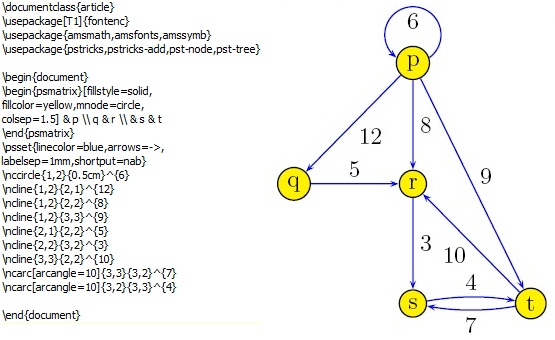
\includegraphics{late.jpg}
\end{center}
\end{enumerate}
\end{itemize}
\newpage

\subsection{TraductorHTML}

En TALFi 1.0 esta clase se encargaba de mostrar un archivo html en un navegador web, con los pasos de la minimizaci\'on de aut\'omatas finitos.\\
\newline
Ahora se ha ampliado su funcionalidad para que muestre tambi\'en la simplificaci\'on de gram\'aticas y la anteriormente mencionada minimizaci\'on, en \LaTeX{}.\\
\newline
Para ello usamos los comandos \LaTeX{} $\bf{tabular}$ y $\bf{hline}$ para dar un formato parecido a las tablas que se generebana en html. De esta manera podemos crear l\'ineas verticales y horizontales para dar aspecto de tabla en \LaTeX{}.\\
\newline
El resto es introducir texto plano y los atributos de las distintas gram\'aticas que se van simplificando.
\newpage
\begin{center}
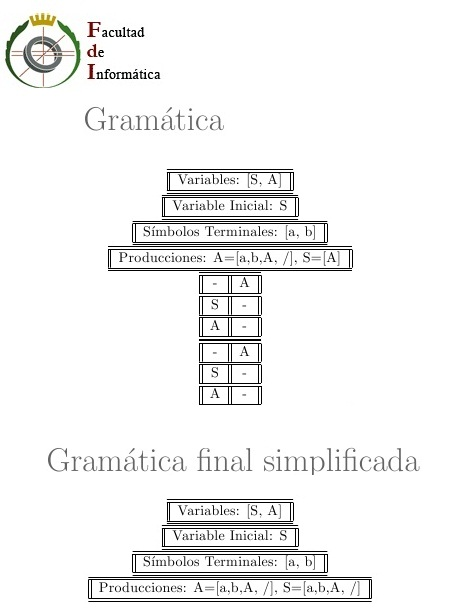
\includegraphics{late3.jpg}
\end{center}
\newpage
\subsection{Entornos \LaTeX{} utilizados}
\begin{itemize}
\item Miktex:
\begin{center}
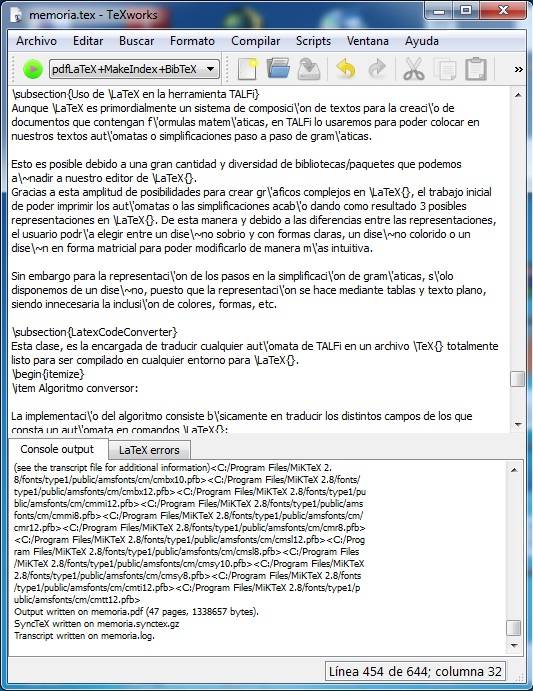
\includegraphics{prog1.jpg}
\end{center}
MiKTeX es una distribuci\'on \TeX{}/\LaTeX{} para Microsoft Windows que fue desarrollada por Christian Schenk.
Las caracter\'isticas m\'as apreciables de MiKTeX son su habilidad de actualizarse por s\'i mismo descargando nuevas versiones de componentes y paquetes instalados previamente, y su f\'acil proceso de instalaci\'on.\\
La versi\'on actual de MiKTeX es 2.8 y est\'a disponible en su \htmladdnormallink{p\'agina oficial}{http://miktex.org/}. Adem\'as, tiene caracter\'isticas que incluyen MetaPost y pdfTeX y compatibilidad con Windows 7. A partir de la versi\'on 2.7 se incluy\'o soporte integrado para XeTeX.

Caracter\'isticas:
\begin{itemize}
\item Es libre y f\'acil de instalar.
\item Incluye m\'as de 800 paquetes con fonts, macros, etc.
\item Tiene un visor propio de archivos dvi denominado Yap.
\item Su c\'odigo es abierto.
\item Posee compiladores \TeX{} y \LaTeX{}, convertidores para generar archivos postscripts (.ps), pdf , html , etc.; y herramientas para generar bibliograf\'ias e \'indices.
\item Posee tres formas de instalaci\'on: peque\~na, mediana y completa.
\end{itemize}
\newpage
\item WinEdt:
\begin{center}
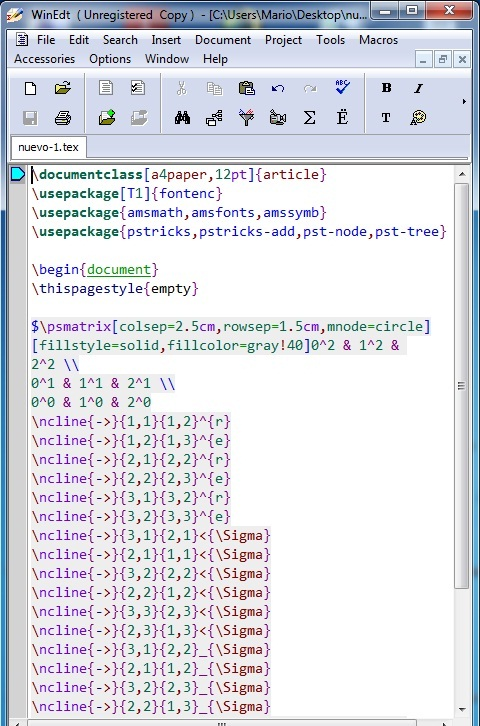
\includegraphics{prog2.jpg}
\end{center}
WinEdt es un editor de textos de gran alcance y versatilidad para Windows, con una fuerte predisposici\'on hacia la creaci\'on de documentos \LaTeX{}.
La \htmladdnormallink{p\'agina de descargas}{http://www.winedt.com/index.html} del sitio web  tiene m\'as informaci\'on sobre WinEdt, \TeX{}, y enlaces a otros programas necesarios para hacer operativo WinEdt en la plataforma Windows.
\end{itemize}

\newpage
\section{Ampliaci\'on del Manual de Usuario}
Antes de que cualquier persona, administrador o no, quiera usar TALFi 2.0, debe conocer dos detalles para poder usar la aplicaci\'on correctamente:\\
\begin{itemize}
\item Si quiere incluir $\epsilon$ en las transiciones, tendr\'a que hacerlo de la misma forma que en TALFi 1.0, con el car\'acter /.
\item Para especificar un blanco en m\'aquinas de Turing, tendr\'a que escribir $\#$.
\item Las direcciones posibles de movimiento en m\'aquinas de Turing son I, D, N para espa\~nol, y L,R,N para ingl\'es. Ambas siempre en may\'usculas.
\item Necesariamente el contenido de la cinta para simular una m\'aquina de Turing debe cargarse en un archivo con extensi\'on ``txt''.
\end{itemize}
Al igual que en la primera versi\'on de TALFi, cuando se pide introducir los s\'imbolos, ya sean de cinta o de alfabeto, en ning\'un caso deben contener espacios y tienen que ir separados por comas.

\newpage
\section{Cambios en la implementaci\'on}
A continuaci\'on enumeraremos brevemente las nuevas clases y los nuevos paquetes creados en este proyecto.\\
Ampliaci\'on de paquetes:

\begin{itemize}
\item Modelo.algoritmos:
\begin{itemize}
\item Clases a\~nadidas:\\AceptaTuring, AutomataP\_to\_GramaticaIC, GIC\_to\_FNG, GIC\_to\_FNChomsky
\item AceptaTuring:\\Contiene el algoritmo que simular\'ia la ejecuci\'on de una m\'aquina de Turing. Recibe el objeto creado para m\'aquinas de Turing y la ruta del archivo que contiene la cinta. Aqu\'i se abre, si ocurriese alg\'un problema no se realiza la simulaci\'on.
\item AutomataP\_to\_GramaticaIC:\\Dado un aut\'omata de pila aplicamos el algoritmo que nos genera su gram\'atica asociada.
\item GIC\_to\_FNC:\\Recibe la gram\'atica que ha generado AutomataP\_to\_GramaticaIC, y la transforma en Forma Normal de Greibach con el algoritmo que utiliza las tablas de reemplazo.
\item GIC\_to\_Chomsky:\\Al igual que GIC\_to\_FNC, genera la correspondiente Forma Normal de Chomsky a partir de la gram\'atica obtenida en AutomataP\_to\_GramaticaIC.
\end{itemize}
\item Modelo.automatas:
\begin{itemize}
\item Alfabeto\_Pila: Interface con las operaciones de alfabetos de pila.
\item AlfabetoPila\_imp:\\Implementa Alfabeto\_Pila y es la clase que como su nombre indica crea y contiene informaci\'on del alfabeto de pila.
\item AlfabetoCinta:\\Crea el alfabeto de cinta de una m\'aquina de Turing.
\item AutomataPila:\\Sirve para crear objetos que identifiquen aut\'omatas de pila.
\item MaquinaTuring:\\Sirve para crear objetos que identifiquen m\'aquinas de Turing.
\end{itemize}
\item Vista.vistaGrafica:
\begin{itemize}
\item AristaGeneral:\\Clase abstracta con todos los atributos y m\'etodos comunes a todos los tipos de aristas.
\item Arista:\\Arista utilizada para todos los aut\'omatas finitos.
\item AristaAP:\\Arista que se utiliza en aut\'omatas de pila.
\item AristaTuring:\\Arista que se emplea en m\'aquinas de Turing.\\
\end{itemize}
\item Vista.vistaGrafica.events:
\item OyenteItemPopupAristaAP:\\Crea el cuadro de di\'alogo cuando se modifica una arista de un aut\'omata de pila.
\item OyenteItemPopupAristaTuring:\\Crea el cuadro de di\'alogo cuando se modifica una arista de una m\'aquina de Turing.
\item OyenteModificaAristaAPActionListener:\\Procesa los nuevos atributos que se han cambiado al modificar la arista de un aut\'omata de pila si se pulsa aceptar con el rat\'on.
\item OyenteModificaAristaTuringActionListener:\\Procesa los nuevos atributos que se han cambiado al modificar la arista de una m\'aquina de Turing si se pulsa aceptar con el rat\'on.
\item OyenteModificaAristaAPKeyAdapter:\\Procesa los nuevos atributos que se han cambiado al modificar la arista de un aut\'omata de pila si se aceptan pulsando Intro.
\item OyenteModificaAristaTuringKeyAdapter:\\Procesa los nuevos atributos que se han cambiado al modificar la arista de una m\'aquina de Turing si se aceptan pulsando Intro.
\end{itemize}
\newpage
Creaci\'on de paquetes:\\
\begin{itemize}
\item Modelo.gramatica:\\
\begin{itemize}
\item Chomsky:\\Crea objetos que representen una gram\'atica en Forma Normal de Chomsky.
\item Gramatica:\\Clase abstracta con los atributos y m\'etodos comunes a todas las gram\'aticas que generamos en esta aplicaci\'on.
\item GramaticaIC:\\Clase que extiende a Gramatica, y cuyos objetos representan la gram\'atica resultante antes de transformarla en ninguna Forma Normal.
\item Greibach:\\Crea objetos que representen una gram\'atica en Forma Normal de Greibach.
\item Produccion:\\Crea los objetos que procesaremos como producciones.
\end{itemize}
\end{itemize}

\newpage
\section{Cambios en la interfaz gr\'afica}
Ante todo hemos de decir que nuestro objetivo ha sido incluir las nuevas funciones de TALFi alterando lo m\'inimo posible el dise\~no que hasta el momento tenia la aplicaci\'on.\\
\begin{itemize}
\item Crear un nuevo aut\'omata de pila / m\'aquina de Turing.\\

Para no saturar m\'as de botones, no hemos incluido uno que fuera un acceso directo para crear un nuevo ejemplo de m\'aquina de Turing o aut\'omata de pila. Si el usuario desea un nuevo ejemplo de estas caracter\'isticas, tendr\'a que dirigirse y hacer click en el apartado ``Archivo'' del men\'u superior:\\
\begin{center}
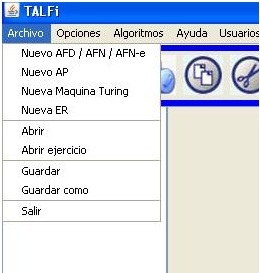
\includegraphics{roci2.jpg}
\end{center}
\item Botones:\\

La segunda novedad son los tres botones para la generaci\'on aleatoria de palabras para aut\'omatas de pila, cargar la cinta inicial de la m\'aquina de Turing y la generaci\'on del c\'odigo en \LaTeX{} del aut\'omata que visualizamos en el canvas.\\ Al comienzo de la aplicaci\'on aparecen los tres desactivados, y seg\'un las \'areas que trabajemos se ir\'an activando si corresponde.\\ Lo mismo ocurre con la secci\'on algoritmos, las opciones est\'an \'unicamente disponibles cuando sea l\'ogico el poder aplicarlas.
\newpage
Men\'u al iniciar la aplicaci\'on:\\
\begin{center}
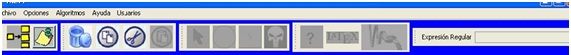
\includegraphics{roci3.jpg}
\end{center}
\begin{center}
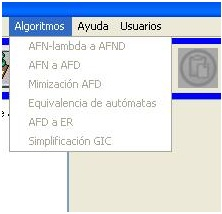
\includegraphics{roci4.jpg}
\end{center}
Muestra de los botones activos en un ejemplo de m\'aquina de Turing:\\
\begin{center}
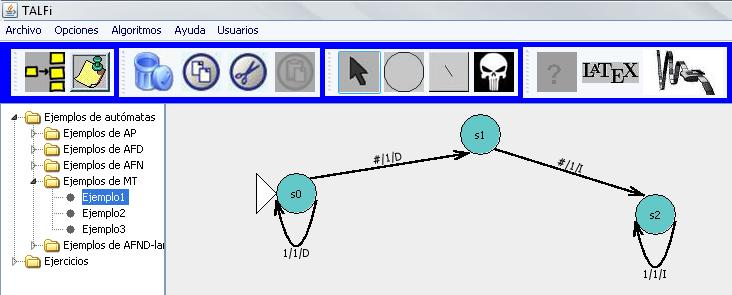
\includegraphics{roci5.jpg}
\end{center}
\newpage
\item Aristas:\\

Ahora las aristas contendr\'an tres campos separados por el car\'acter / :\\
s\'imbolos de entrada o s\'imbolos de cinta, cima de pila actual o s\'imbolo que reemplazar\'a al que actualmente est\'a en la cinta, y la transici\'on de la pila o la direcci\'on hacia la que se desplazar\'a la cabeza lectora de la cinta de Turing, ya se trate de aut\'omatas de pila o m\'aquinas de Turing.\\ En consecuencia, necesitaremos tres campos distintos a modificar cuando necesitemos modificar una arista ya dibujada en el canvas.\\

Cuadro de di\'alogo que aparece al modificar una arista de un aut\'omata de pila:\\
\begin{center}
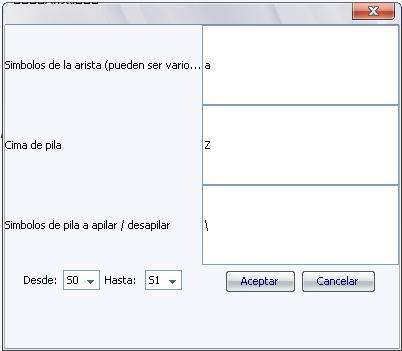
\includegraphics{roci6.jpg}
\end{center}
\end{itemize}

\begin{thebibliography}{XXX}
\bibitem{}Hopcraft, Motwani, Uliman.\\
``Introducci\'on a la teor\'ia de aut\'omatas. Lenguajes y computaci\'on''\\
Addison Wesley 2002.
\bibitem{}J. G. Brookshear.\\
Teor\'ia de la Computaci\'on: Lenguajes Formales, Aut\'omatas y Complejidad.\\
Addison-Wesley Iberoamericana, 1993.
\bibitem{}J.C. Martin.\\
Introduction to Languages and the Theory of Computation\\
McGraw-Hill, 1997, (Segunda edici\'on).
\bibitem{}D.C. Kozen\\
Automata and Computability\\
Springer Verlag, 1997.
\bibitem{}H.R. Lewis, C.H. Papadimitriou\\
Elements of the Theory of Computation\\
Prentice Hall, 1988, (Segunda edici\'on).
\bibitem{}P. Isasi, P. Mart\'inez, D. Borrajo\\
Lenguajes, Gram\'aticas y Aut\'omatas, un enfoque pr\'actico.\\
Addison-Wesley, 1997.
\bibitem{}Dean Kelley.\\
``Teor\'ia de Aut\'omatas y Lenguajes Formales''.\\
Prentice Hall, 1997.
\bibitem{}\htmladdnormallink{http://es.wikipedia.org}{http://es.wikipedia.org}
\end{thebibliography}

\end{document} 